\chapter{Results}\label{sec:results}

\section{Filtering out noise}\label{sec:noise}
After the tracking and stitching steps are completed, the algorithm results can
still be improved by filtering the results. A large improvement was
achieved by requiring a certain sea surface temperature at TC genesis.
\subsection*{Sea Surface Temperature Criterion}
As outlined in Sec.~\ref{sec:physics}, the TCs need warm ocean water as an
energy source, when they form. It has been shown that the large
majority has an SST over 25.5\degree C \cite{sst-paper}. Therefore it is
expected that no reasonable TCs are filtered out when requiring a genesis SST
of at least 24\degree C. However, as can be seen in Fig.~\ref{fig:sst-effect},
a large part of the unwanted tracks in the North of the domain are removed.
% TODO ?? use figures here and in general with reasonable and elaborated parameters only
\begin{figure}[!htb]
	\begin{minipage}[t]{0.48\textwidth}
		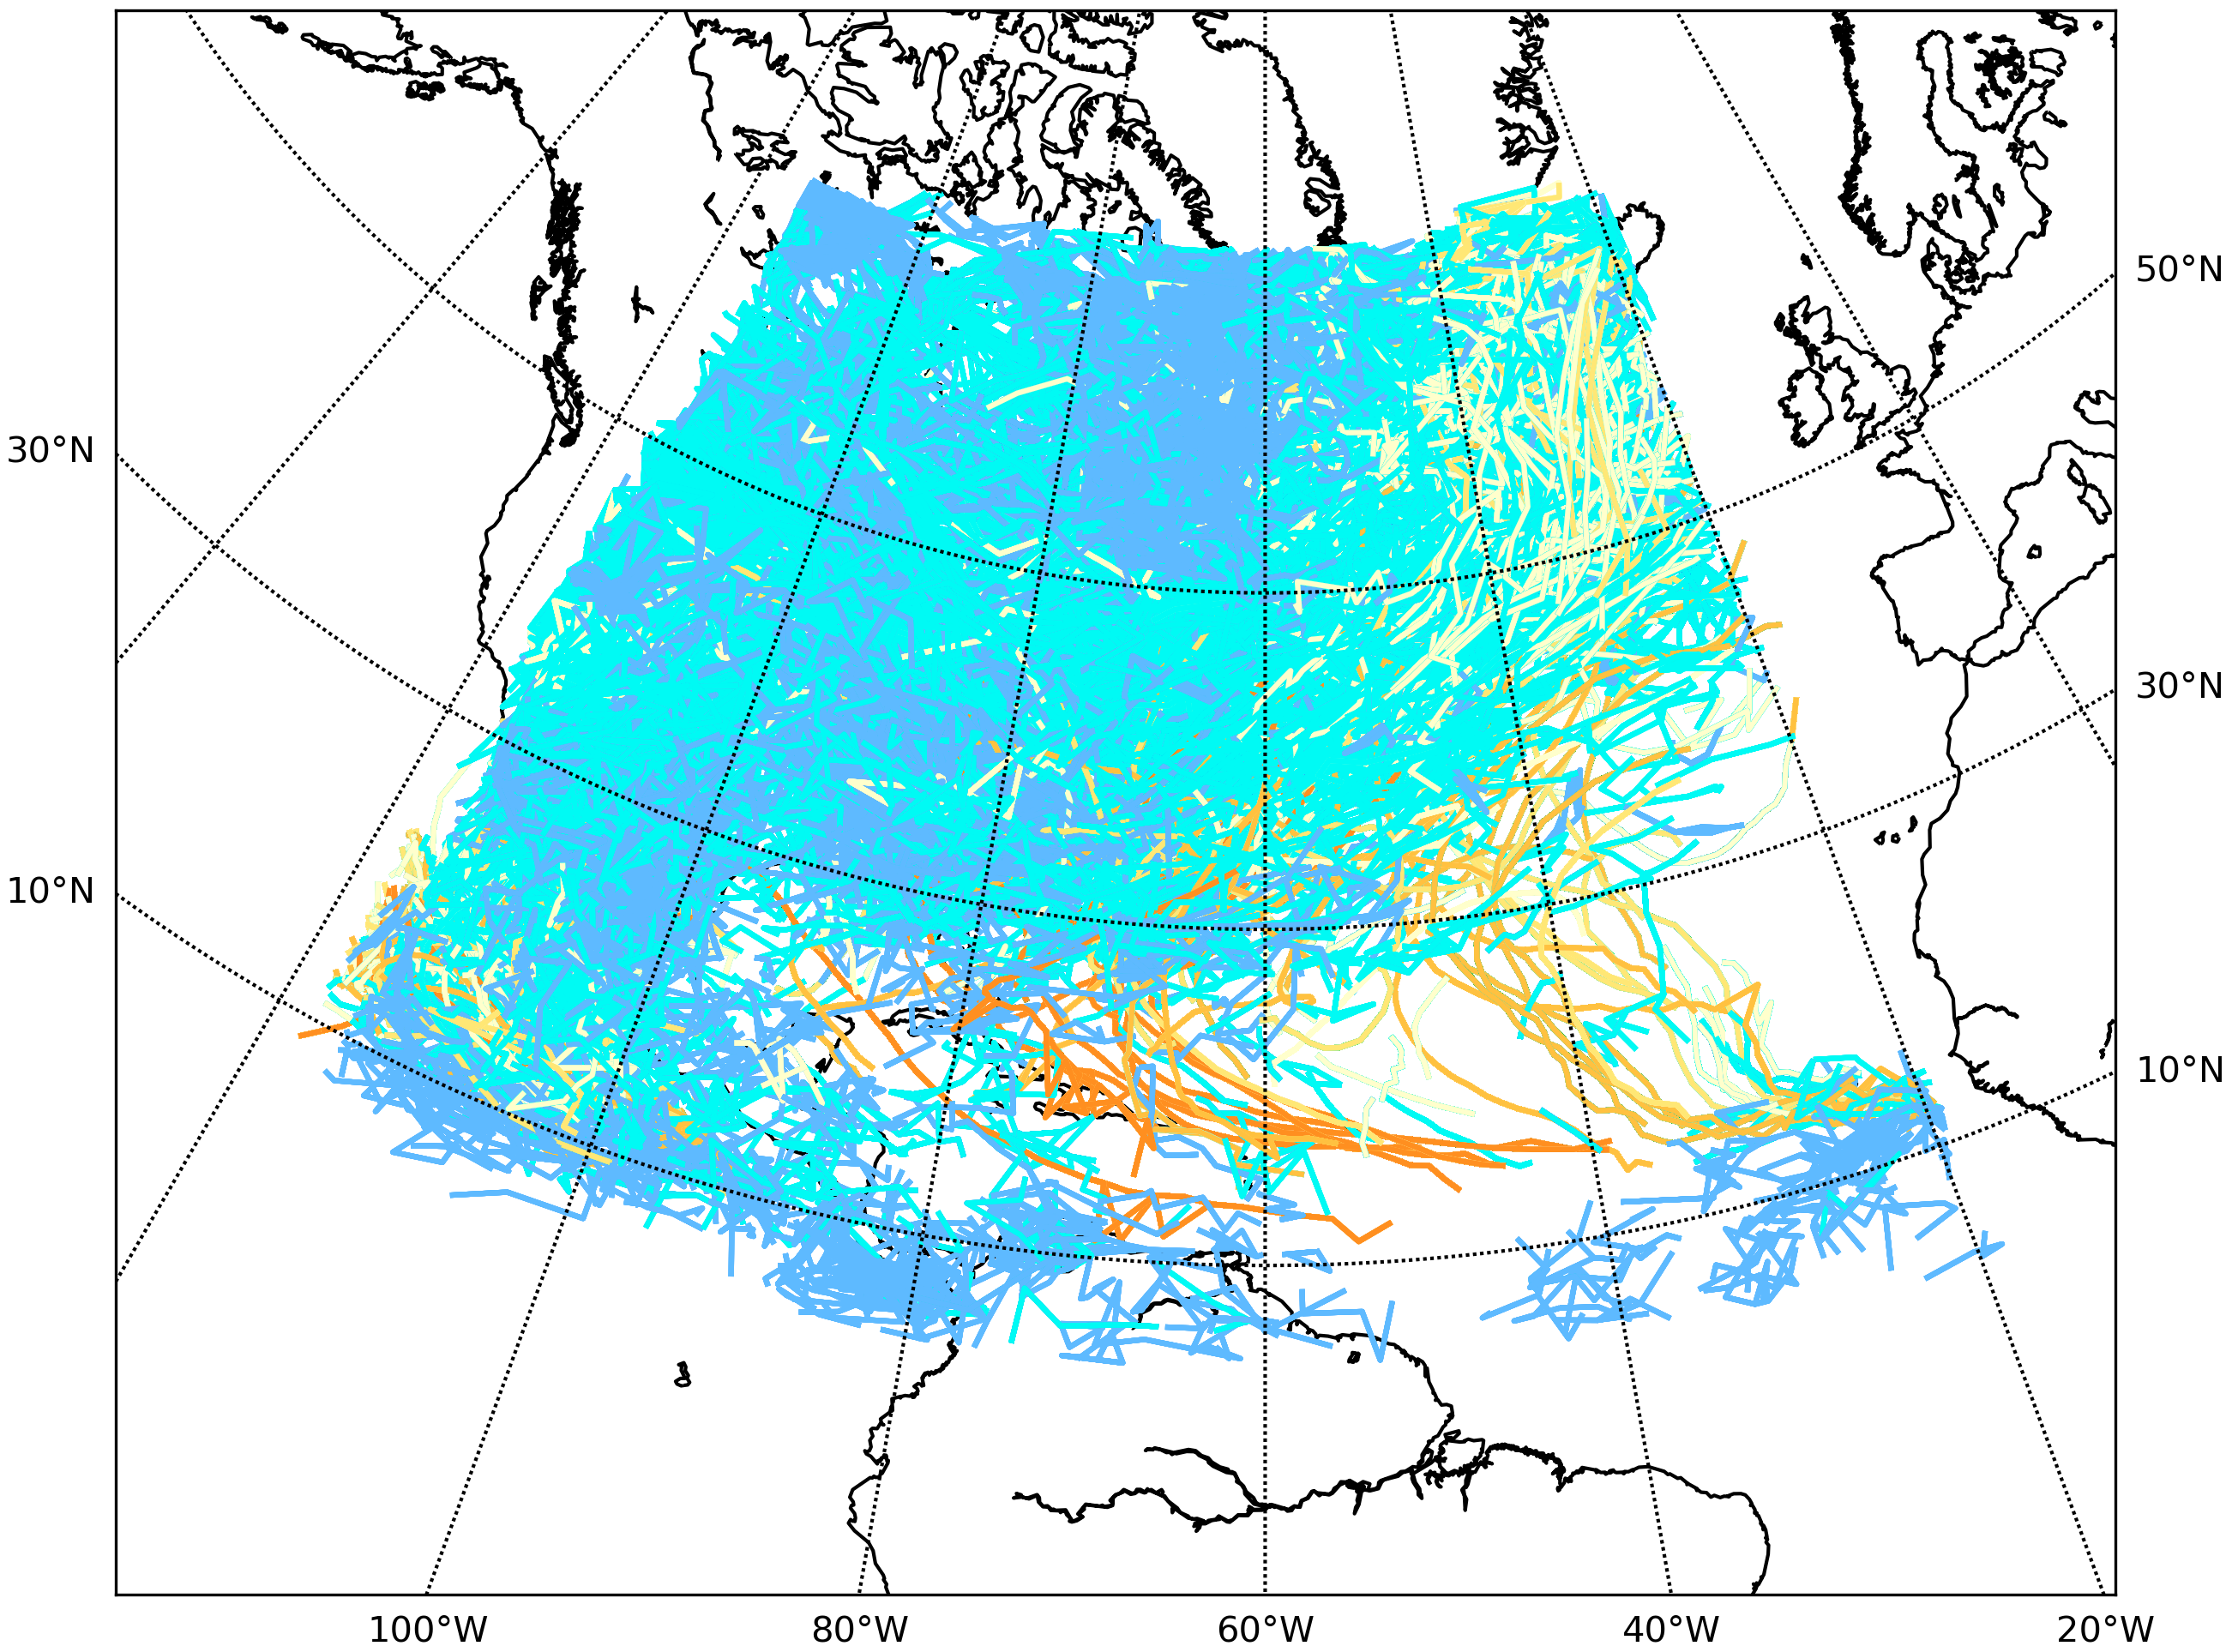
\includegraphics[width = \textwidth]{img/all_tracks.png}
	\end{minipage}
	\hfill
	\begin{minipage}[t]{0.48\textwidth}
		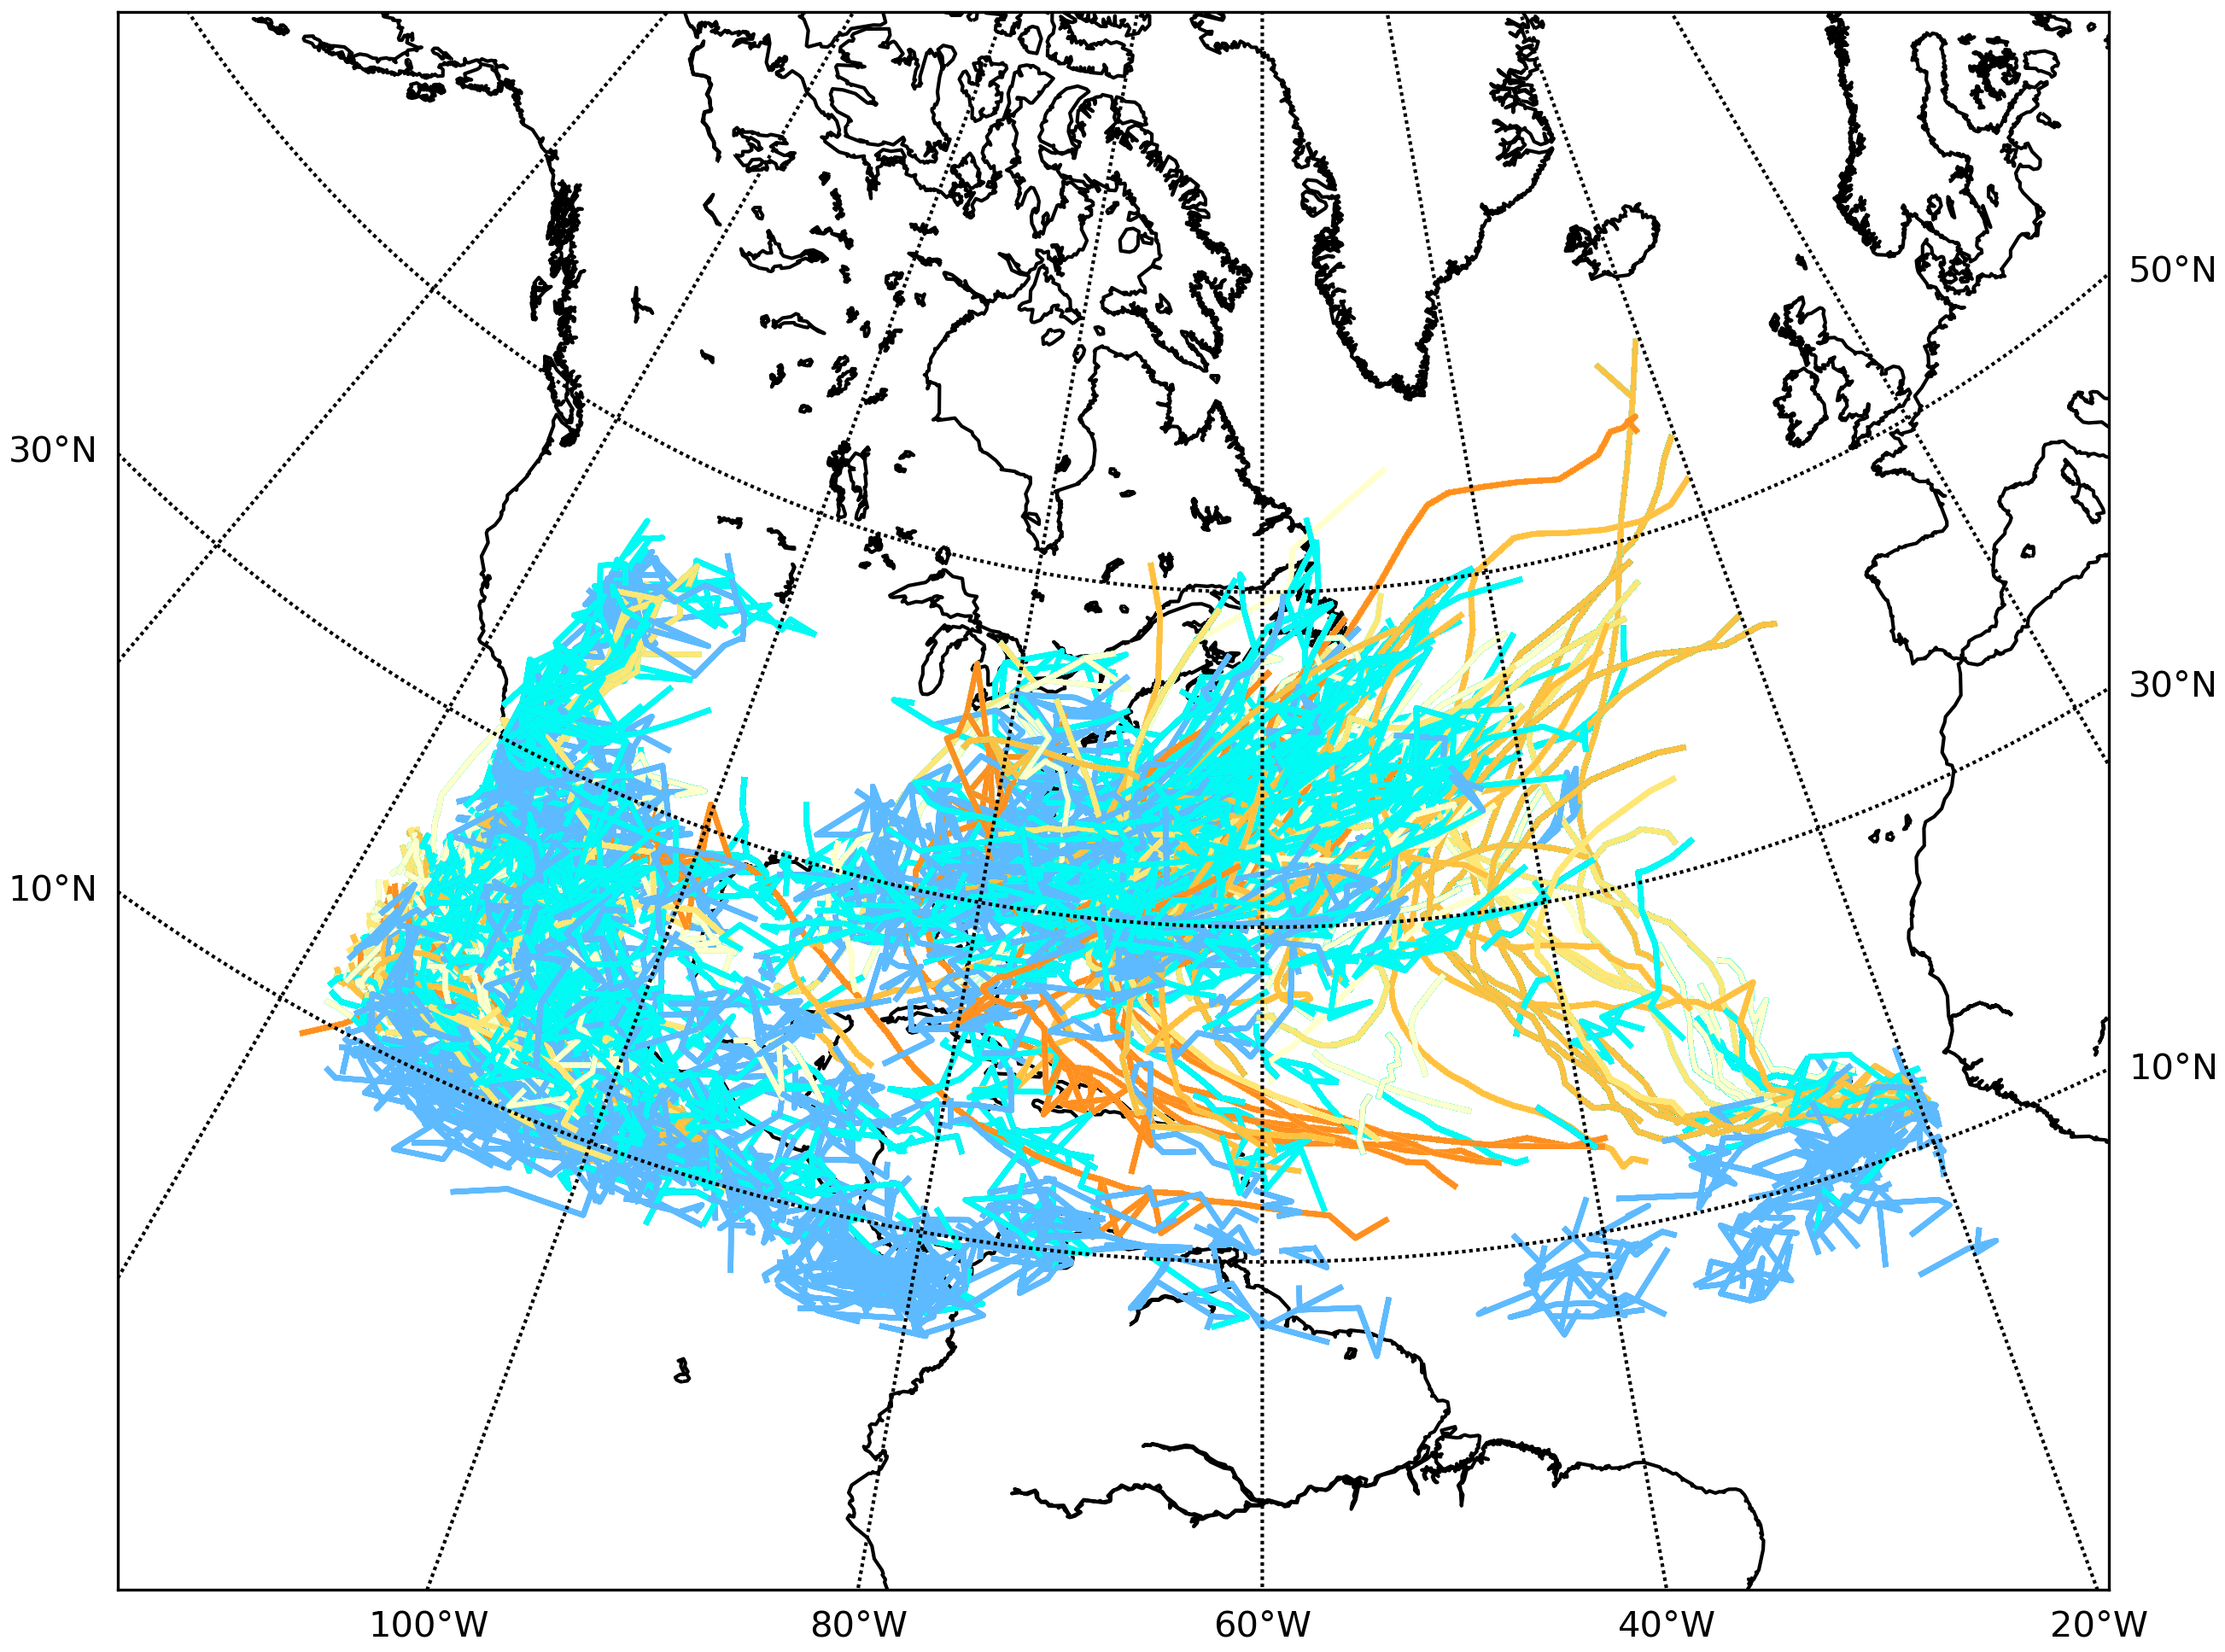
\includegraphics[width = \textwidth]{img/all_tracks_sst.png}
	\end{minipage}
	\caption{Comparison of all tracks without and with the SST criterion on the left and right}
	\label{fig:sst-effect}
\end{figure}

\subsection*{Analysing geographically unreasonable tracks}
Even with the application of the SST-criterion, unreasonable TC tracks remain. For instance the tracks over Wyoming shown in Fig.~\ref{fig:rogue-tracks} should not be so frequent. Interestingly these TCs develop over the Great Salt Lake. To determine the parameters responsible for this, the 20 parameter combinations that account for the large majority of these, share the common feature that they all correspond to the same weak warm core criterion. They had a \textbf{temdif} of \unit[0.5]{\degree C} and a \textbf{temdis} of \unit[400]{km}. Therefore if only a very low temperature difference is required for an area that can be larger than smaller-sized TCs, low pressure systems that do not correspond to tropical cyclones are tracked. While this may not be surprising, it does emphasise the importance of a well-trimmed warm core criterion.
\begin{figure}[!htb]
	\centering
	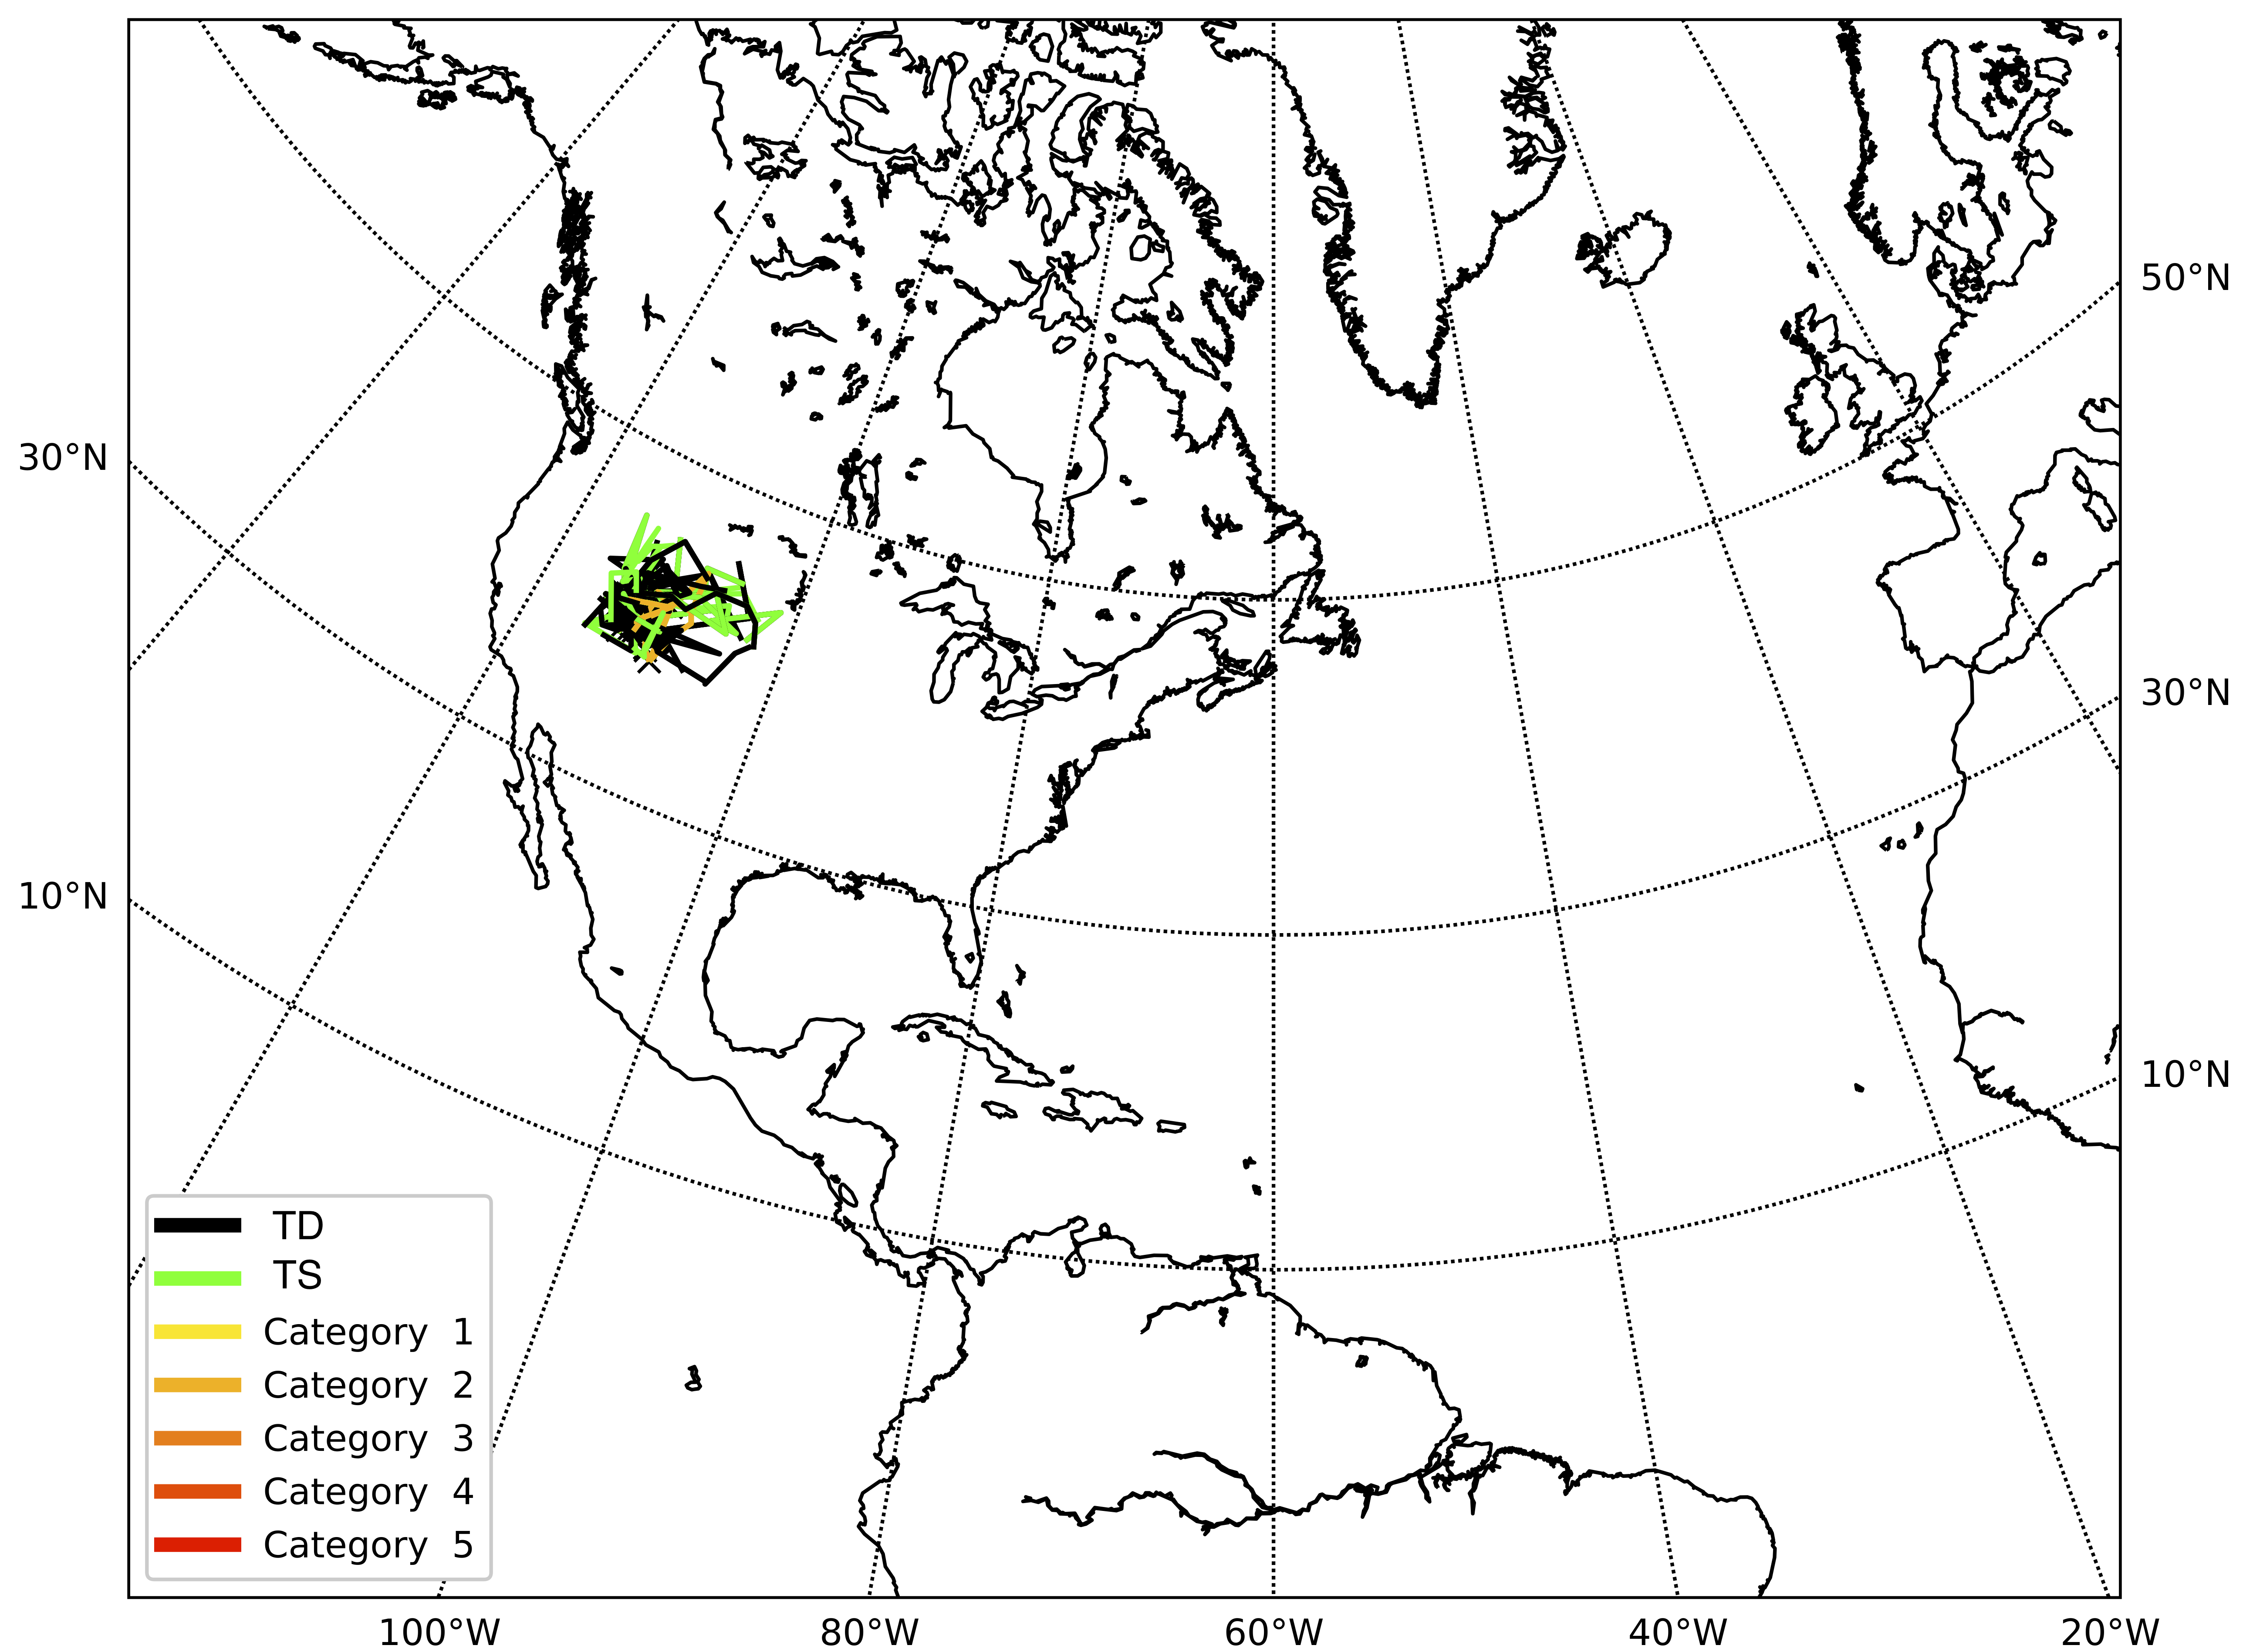
\includegraphics[width=0.5\textwidth]{img/rogue_tracks.png}
	\caption{Set of unreasonable tracks over Wyoming and the surrounding states.}
	\label{fig:rogue-tracks}
\end{figure}
\section{Validating Results}
In Sec.~\ref{sec:noise}, it was found that with a sufficiently strong warm core condition the tracks appear in reasonable areas. Before comparing the algorithm output for different parameter combinations, it still remains to be shown that the produced tracks actually follow TCs and not other low pressure systems. For this purpose, ten different storms were randomly chosen. For these storms the radial, tangential and vertical wind and the sea level pressure were visualised in the azimuthal mean. It was found that all storms qualitatively exhibit the physically expected structure that was described in Sec.~\ref{sec:physics}. The resulting plots for a representative storm can be seen in Fig.~\ref{fig:azimean}.

\begin{figure}[!htb]
	\centering
	\begin{subfigure}{.5\linewidth}
		\centering
		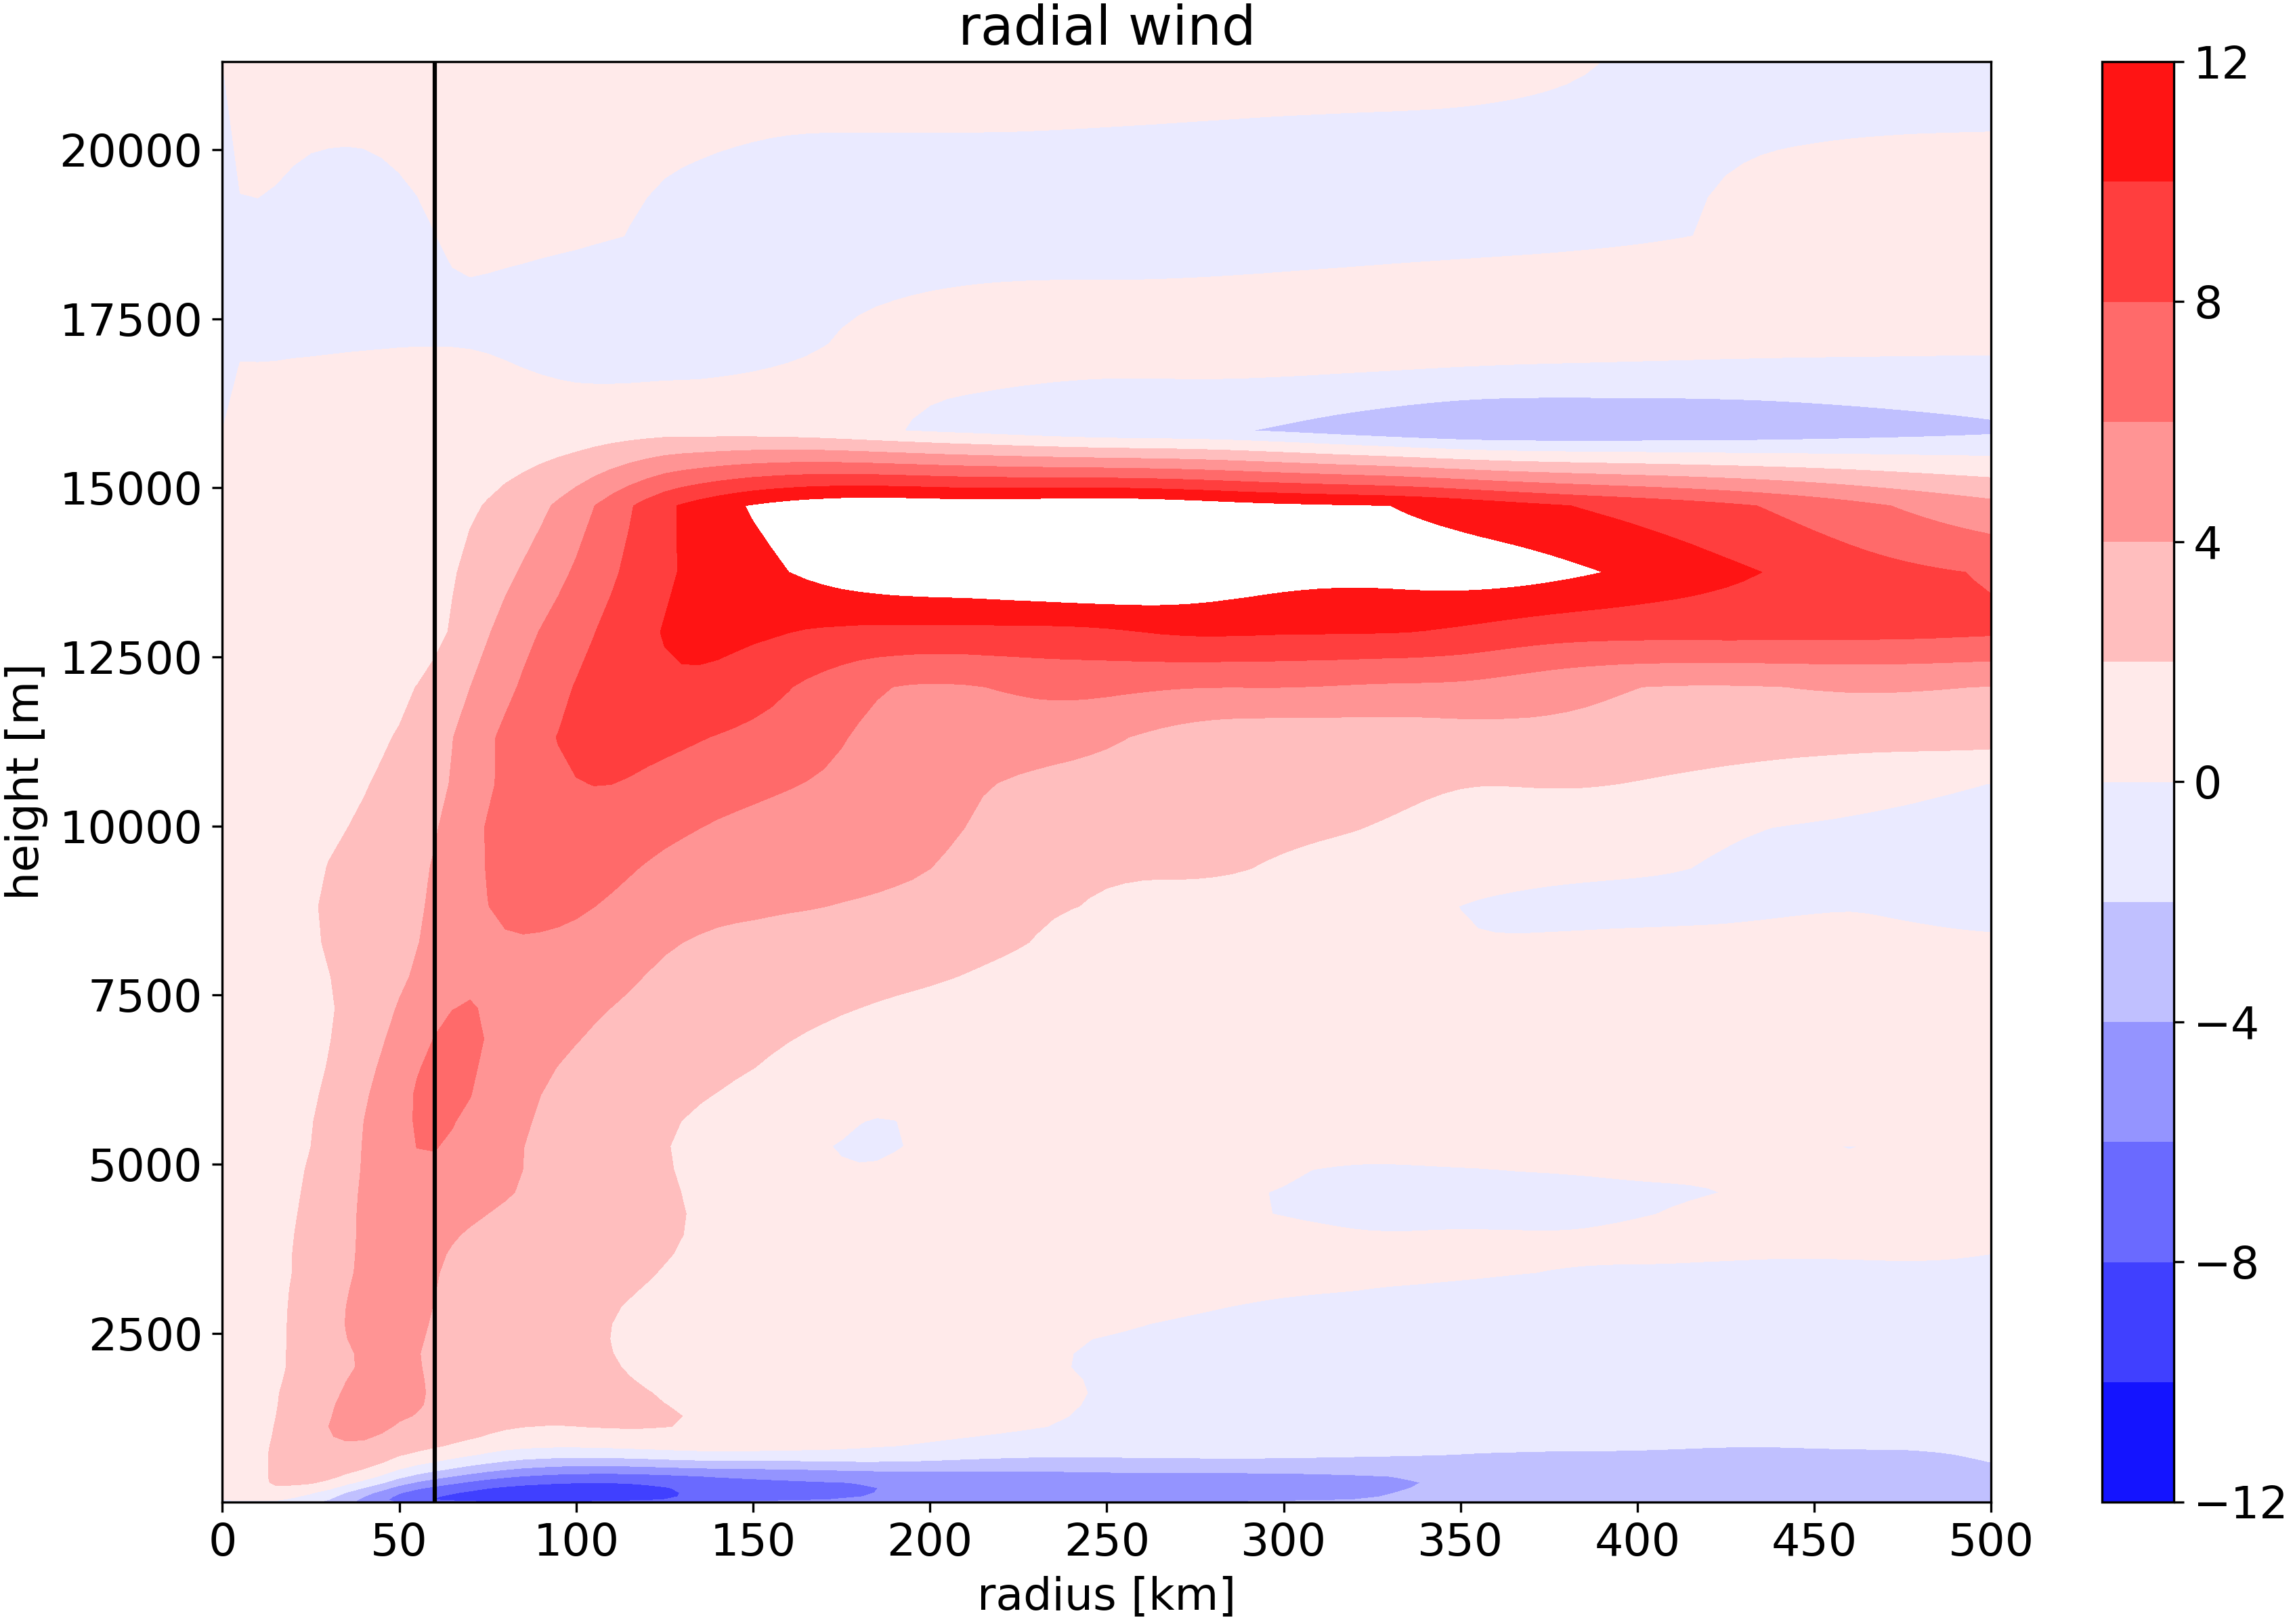
\includegraphics[width=0.85\linewidth]{img/0299554radwind20130905T120000Z_redo.png}
	\end{subfigure}%
	\begin{subfigure}{.5\linewidth}
		\centering
		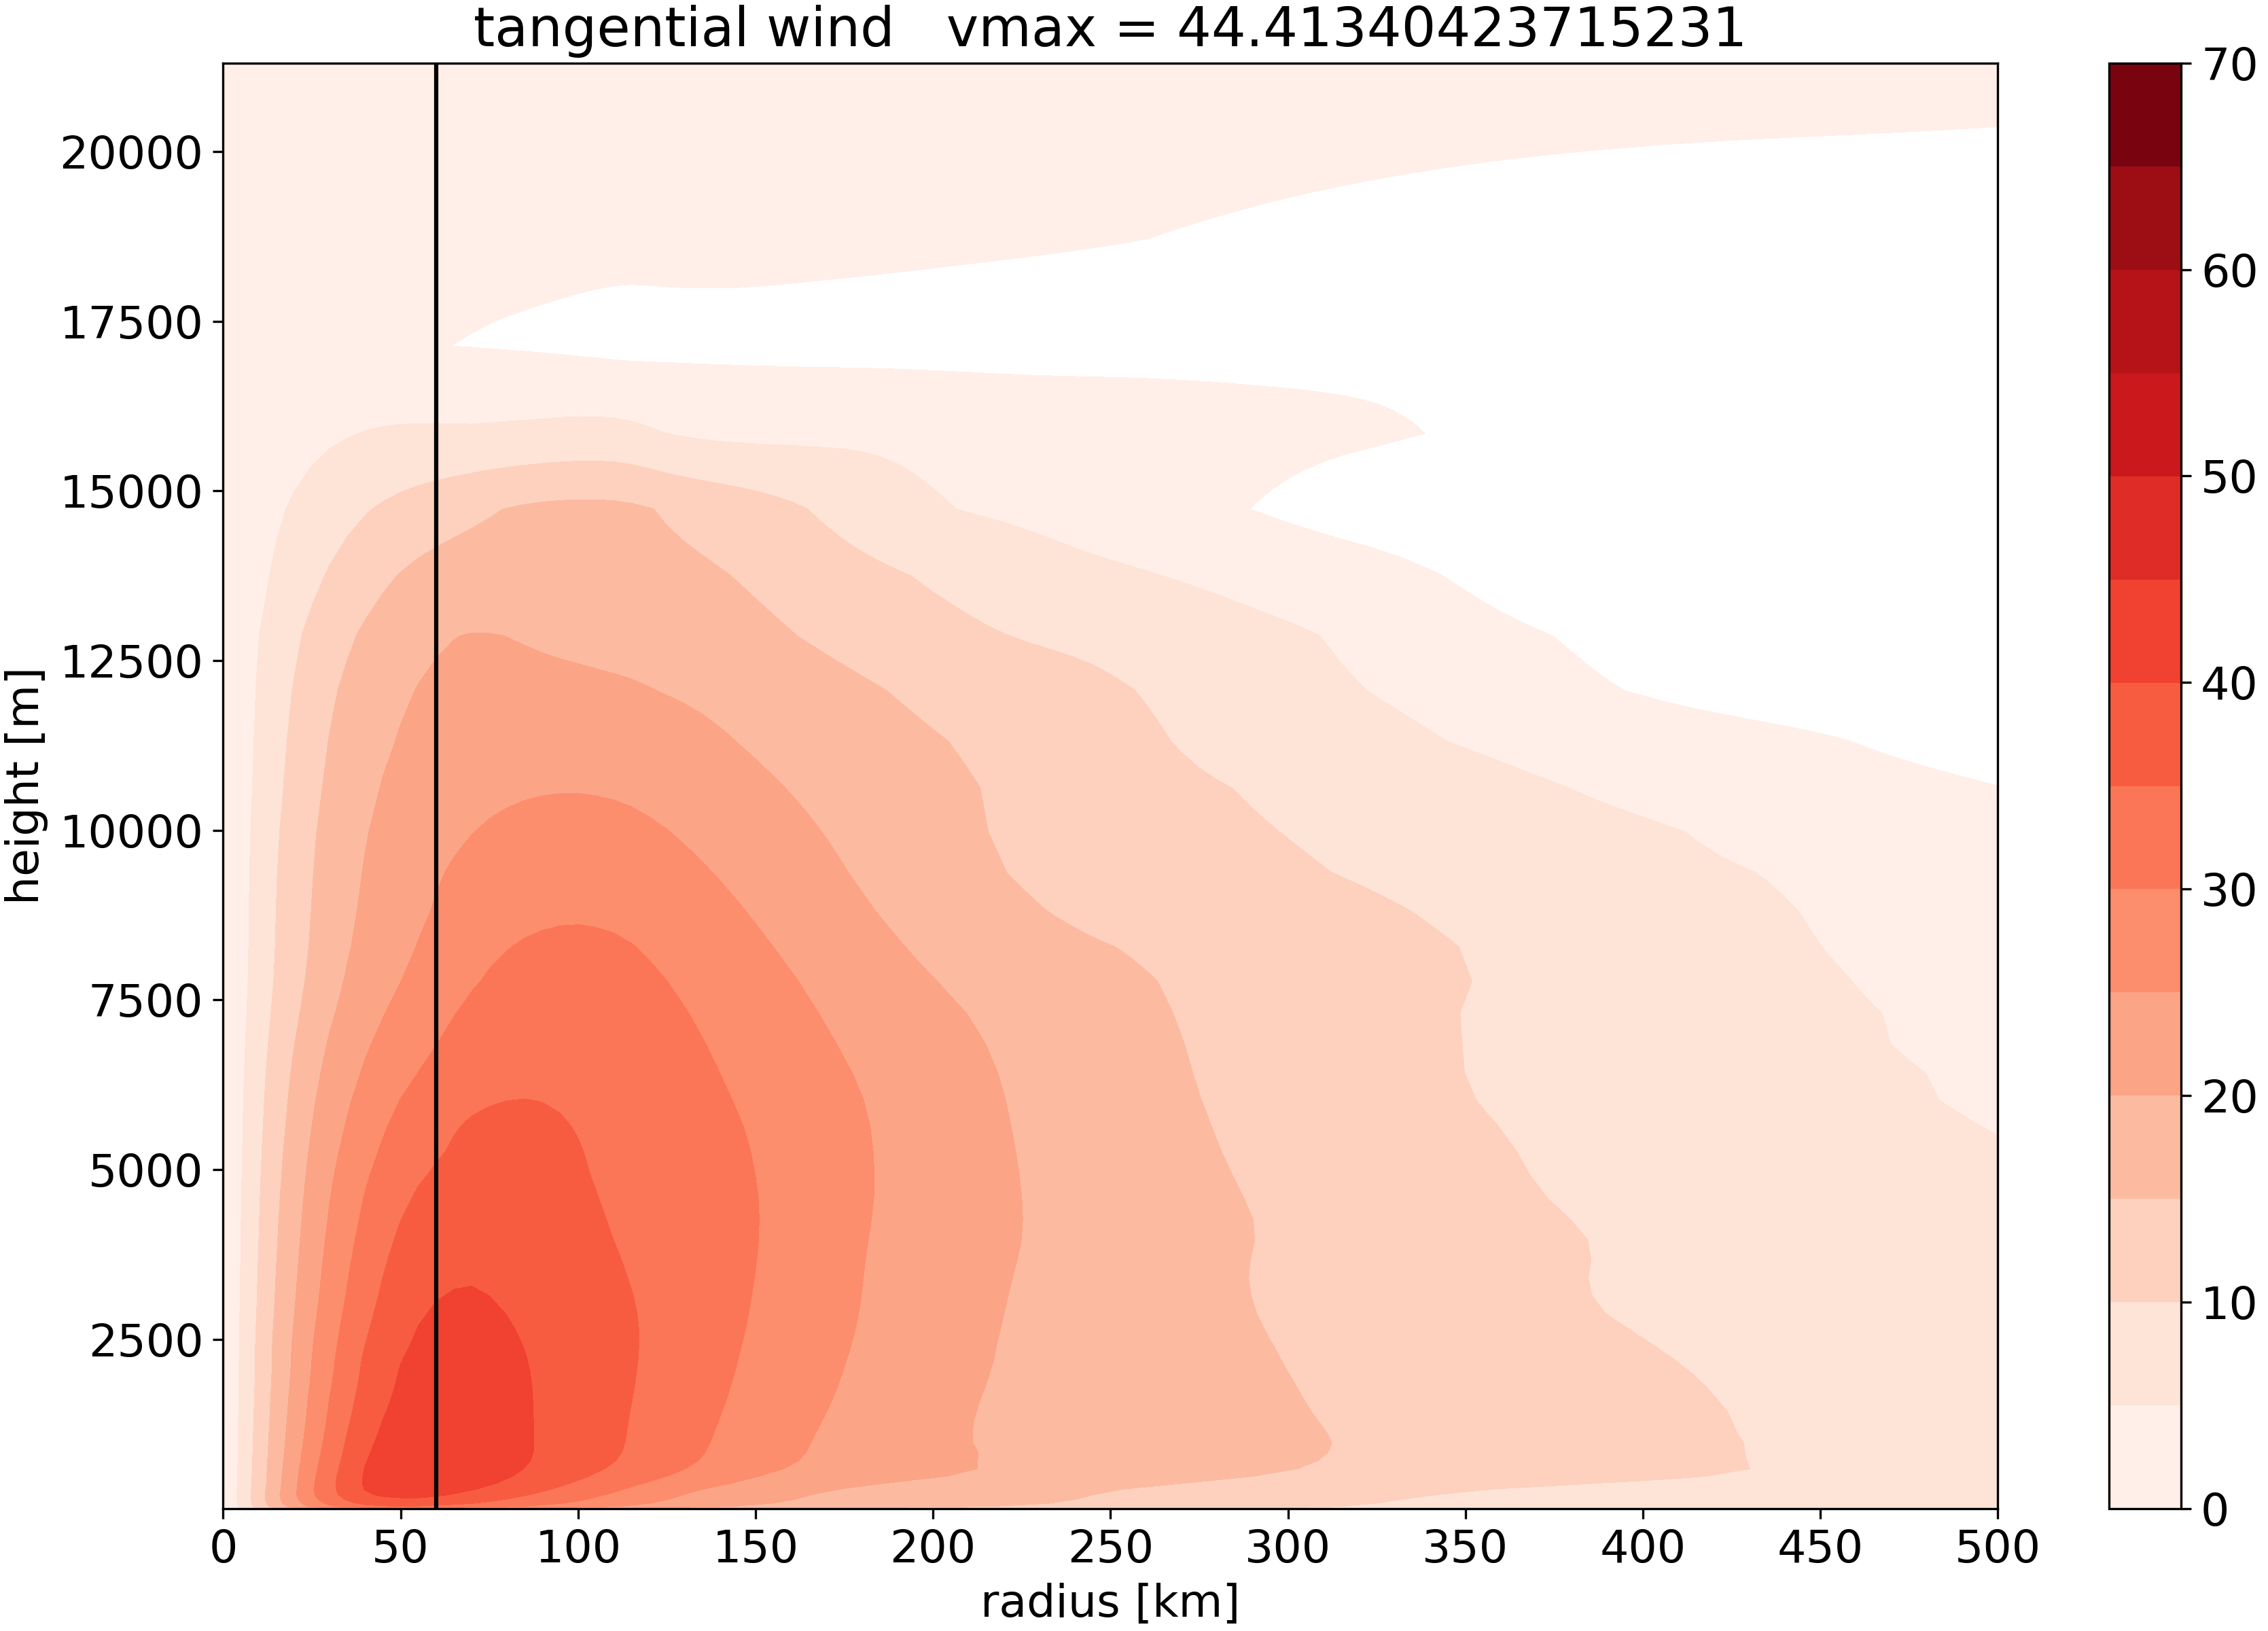
\includegraphics[width=0.85\linewidth]{img/0299554tanwind20130905T120000Z_redo.png}
	\end{subfigure}
	\begin{subfigure}{.5\linewidth}
		\centering
		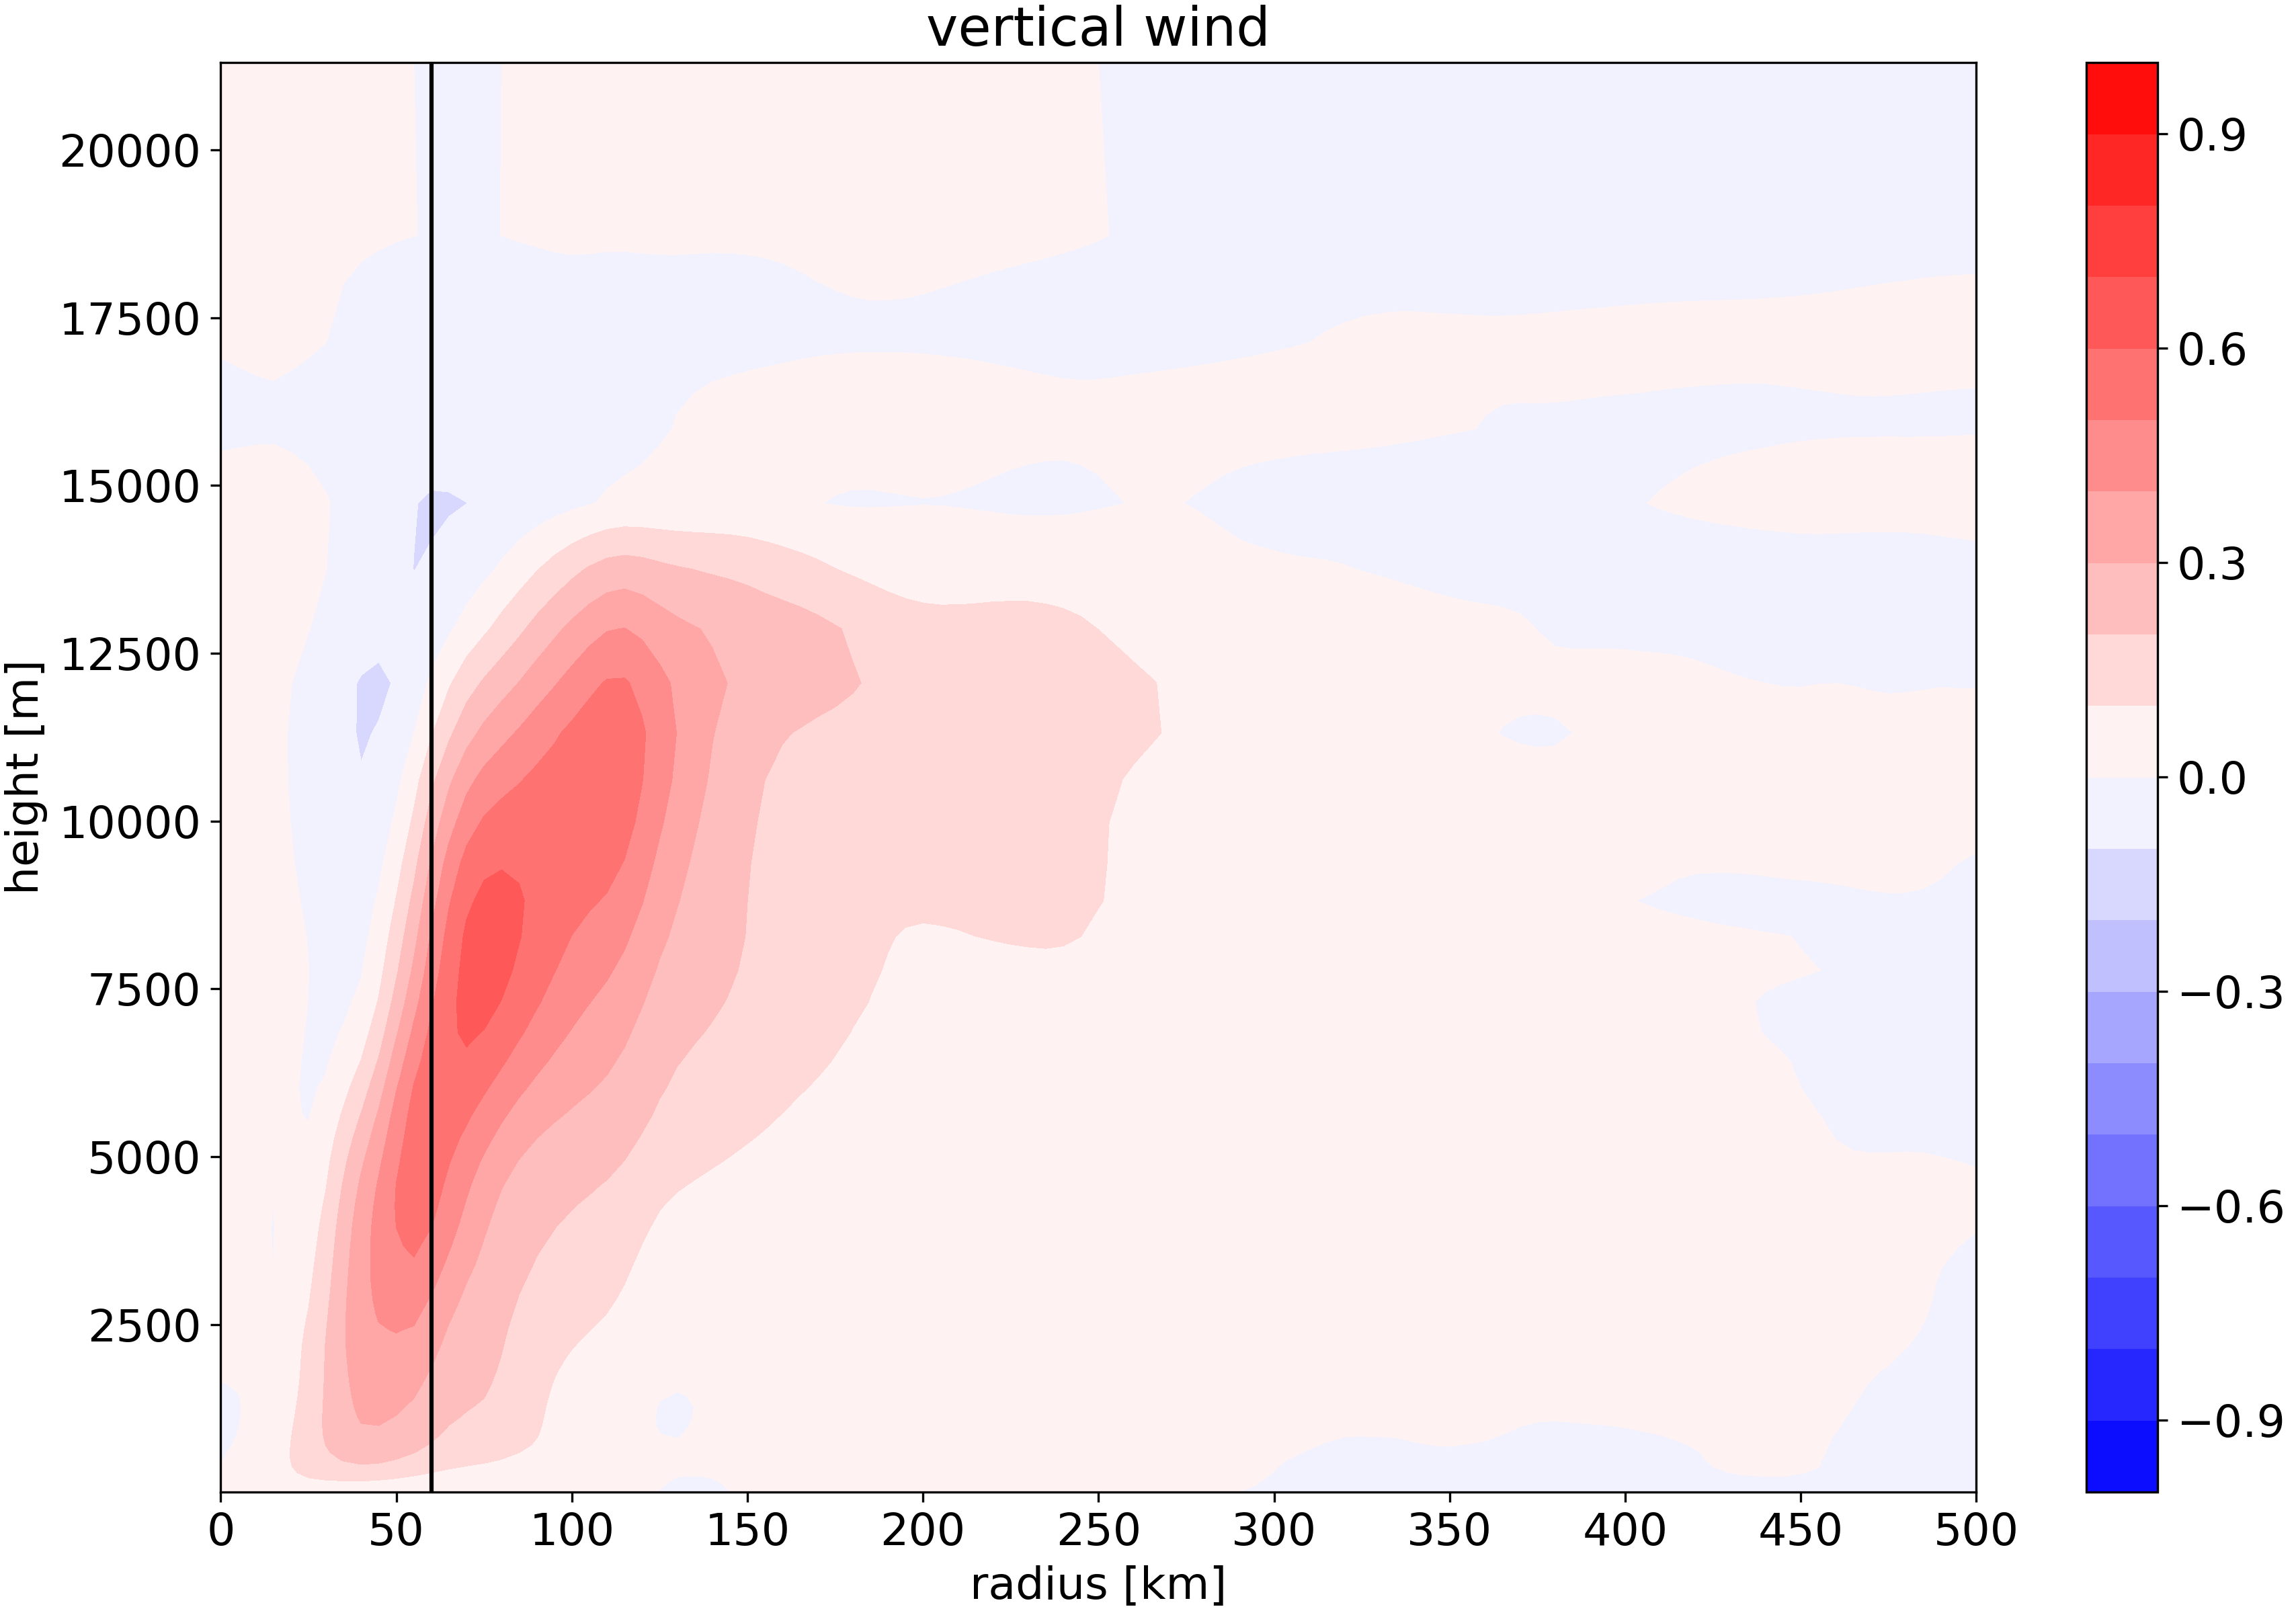
\includegraphics[width=0.85\linewidth]{img/0299554verwind20130905T120000Z_redo.png}
	\end{subfigure}%
	\begin{subfigure}{.5\linewidth}
		\centering
		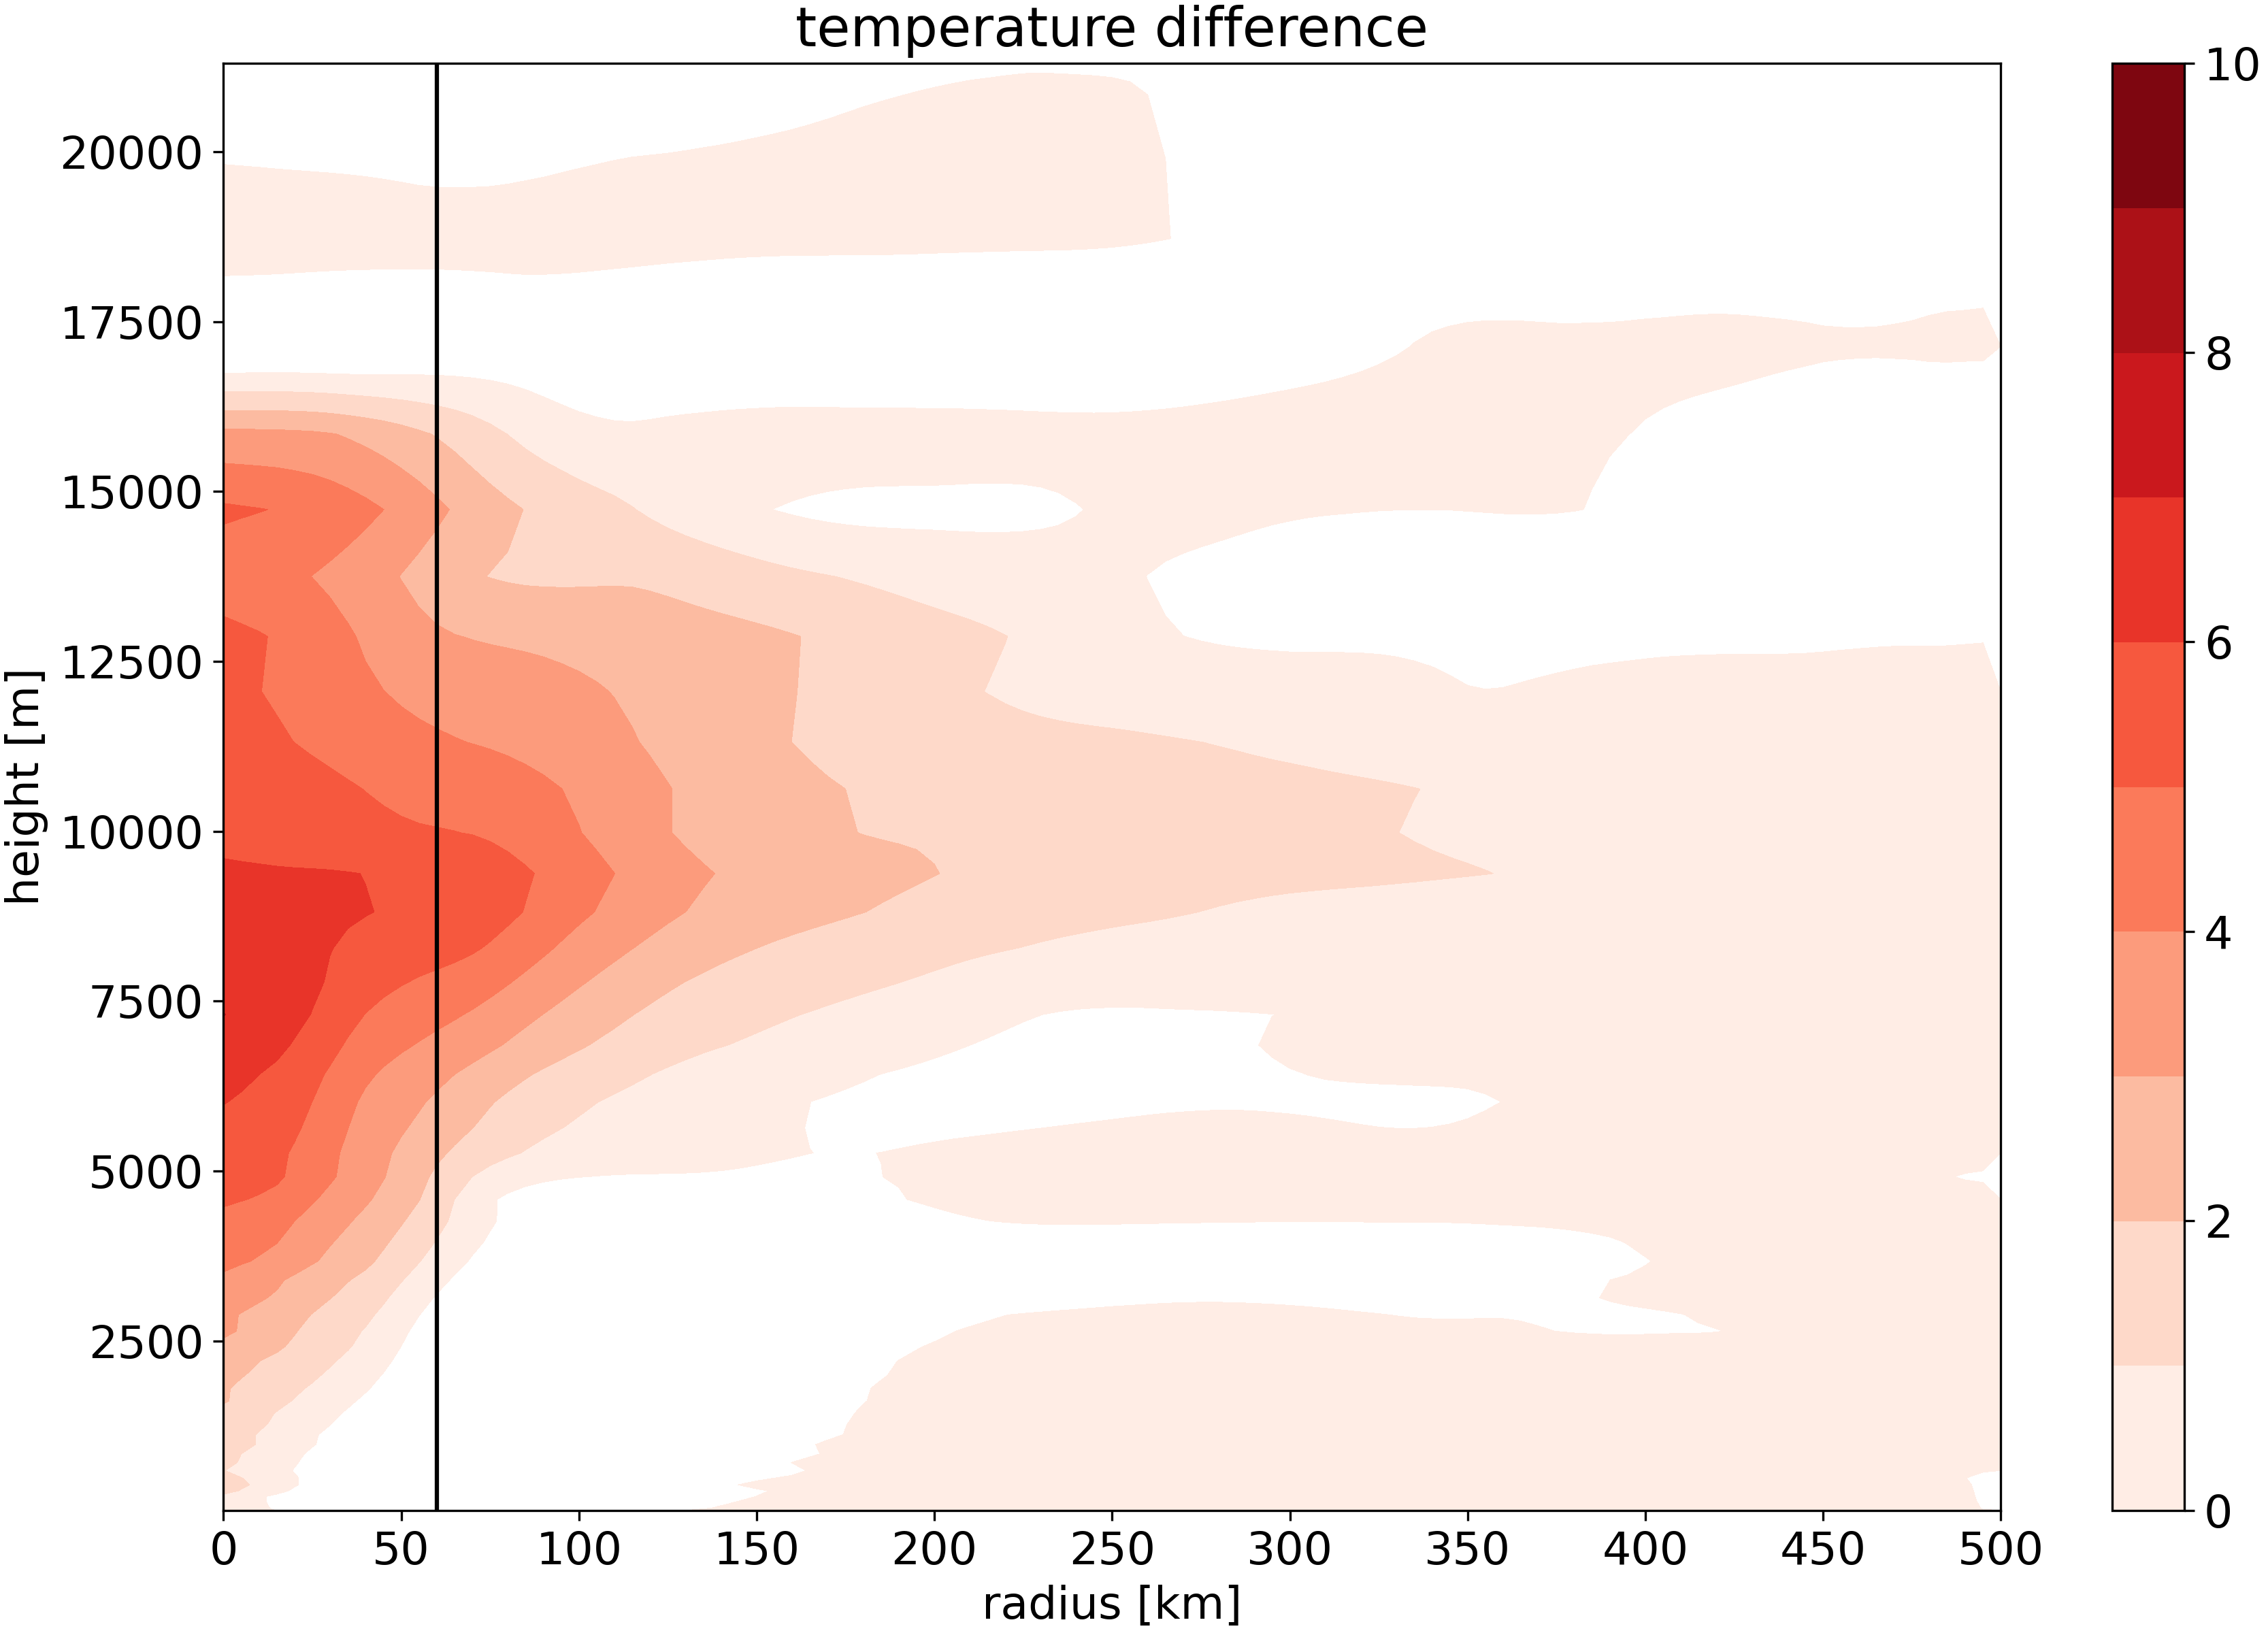
\includegraphics[width=0.85\linewidth]{img/0299554temp20130905T120000Z_redo.png}
	\end{subfigure}
		\begin{subfigure}{.49\linewidth}
		\centering
		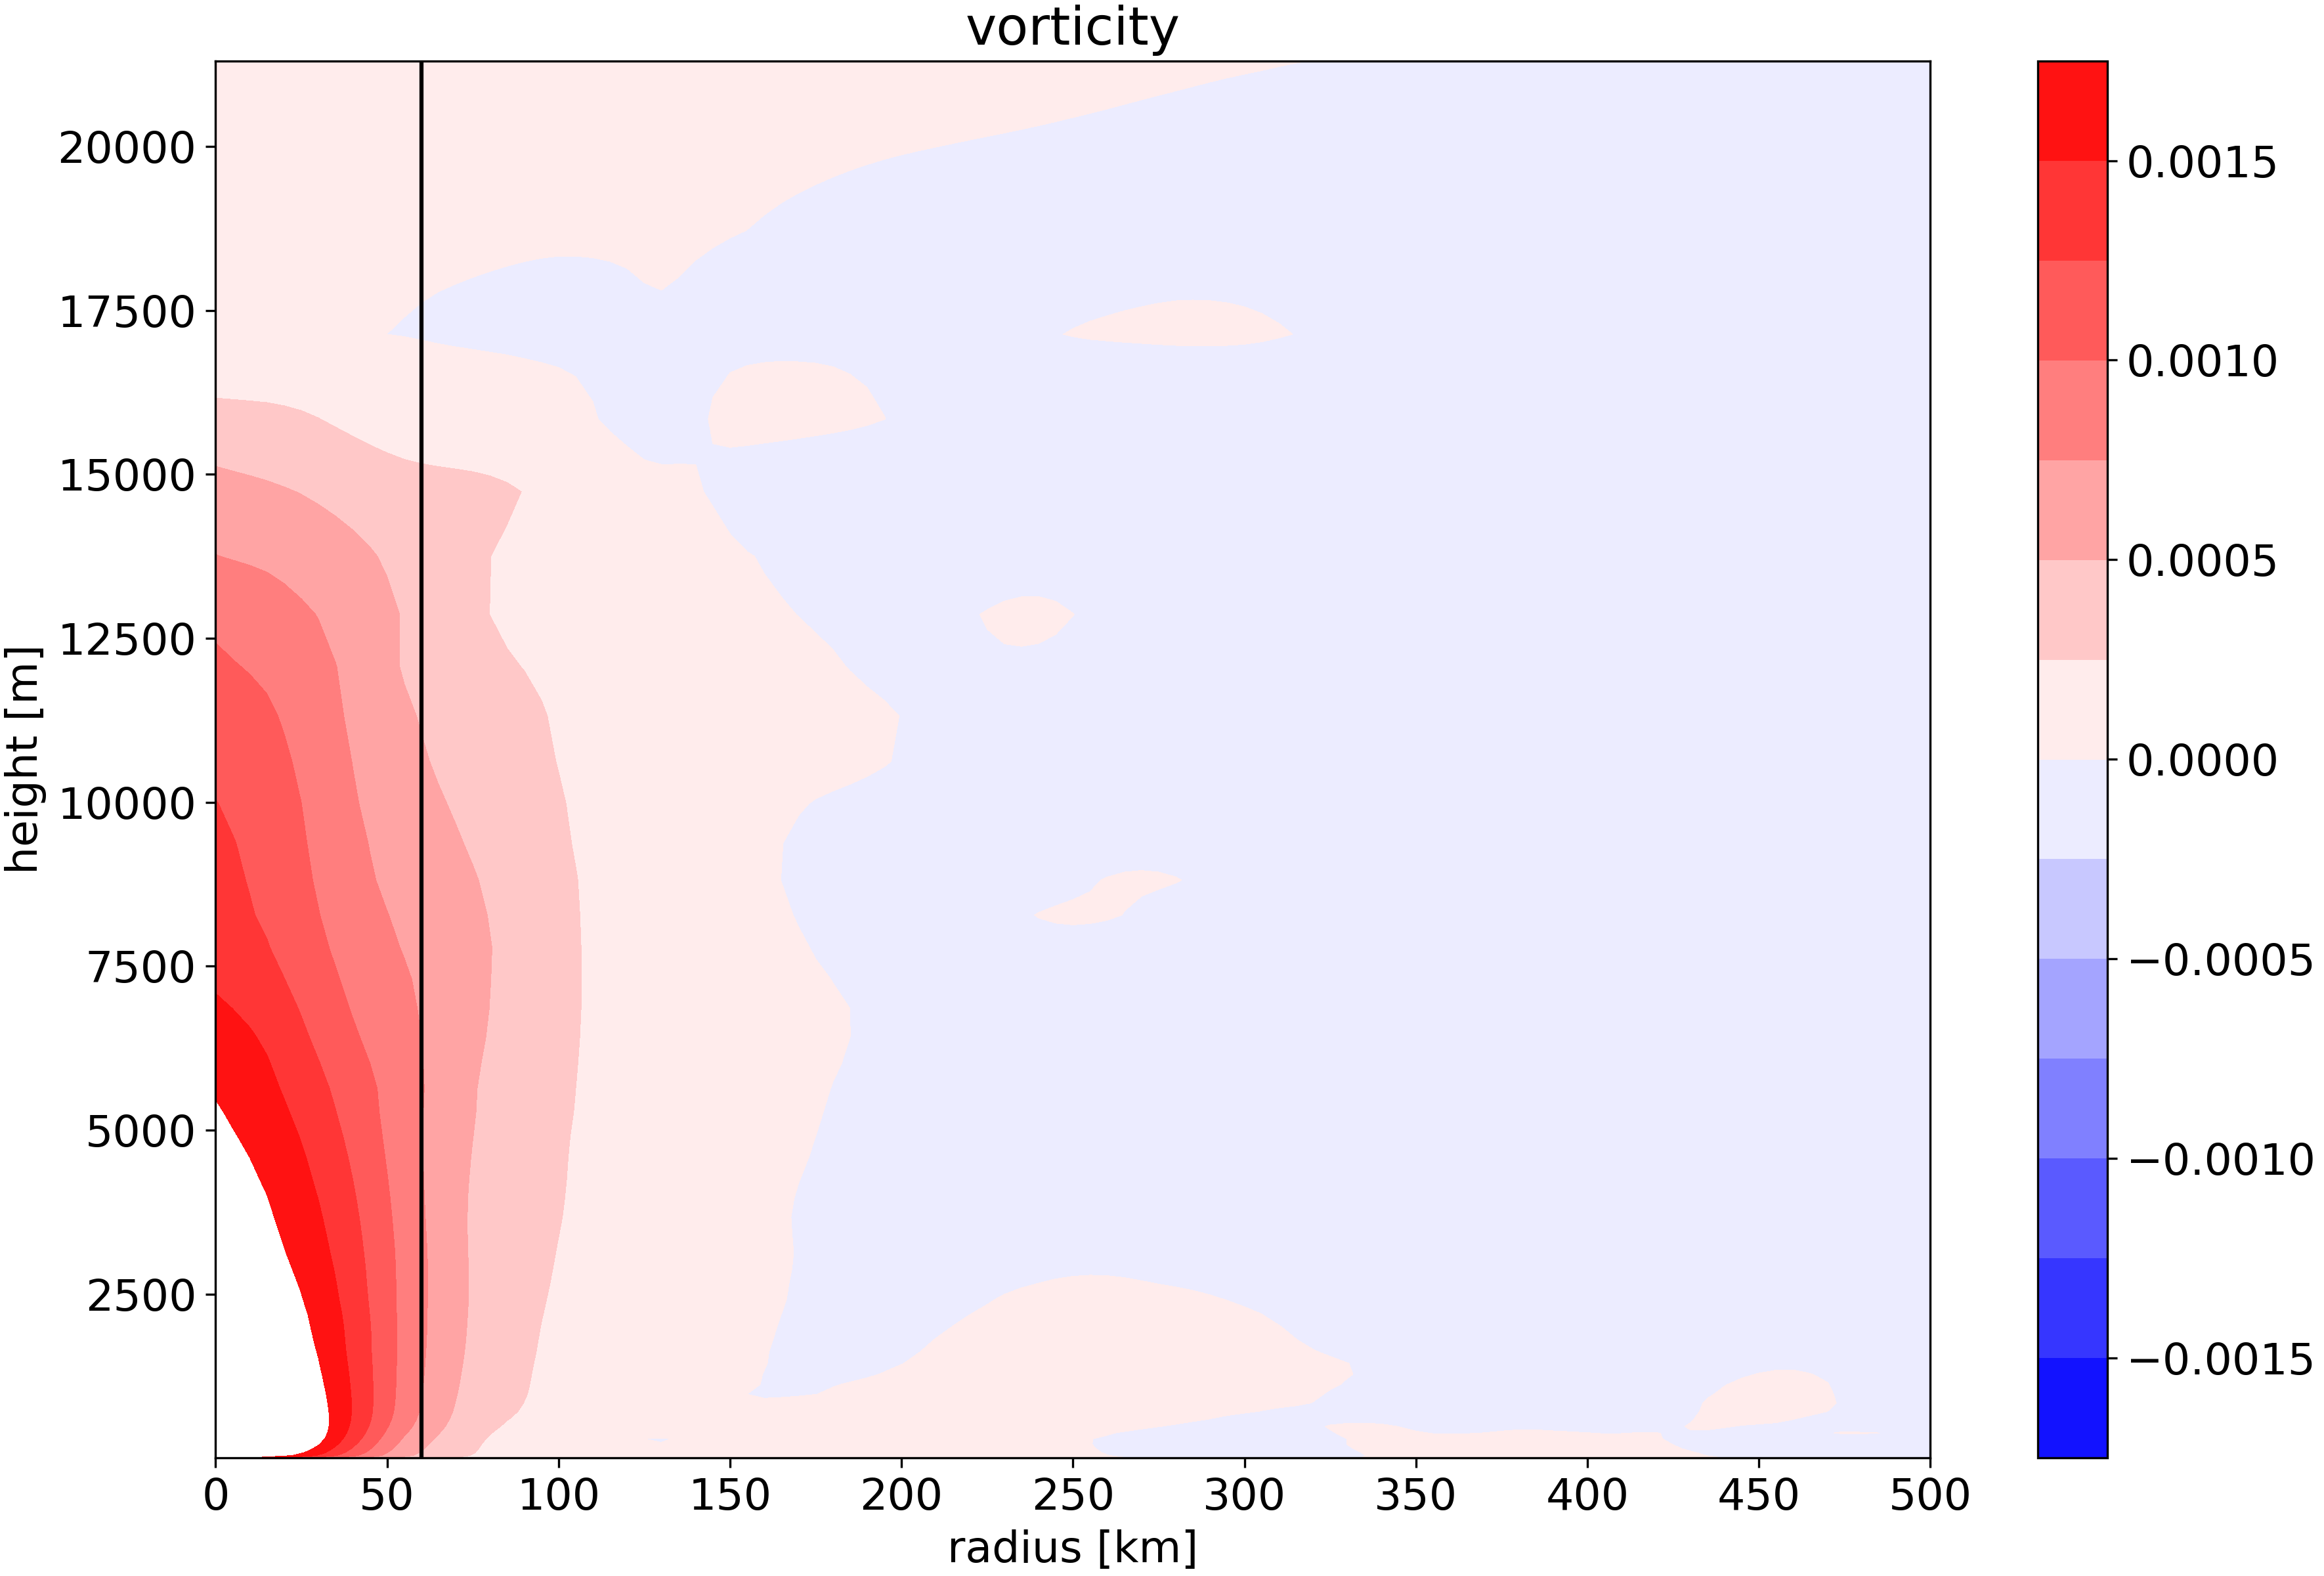
\includegraphics[width=0.85\linewidth]{img/0299554vor20130905T120000Z_redo.png}
	\end{subfigure}
	\begin{subfigure}{.49\linewidth}
		\centering
		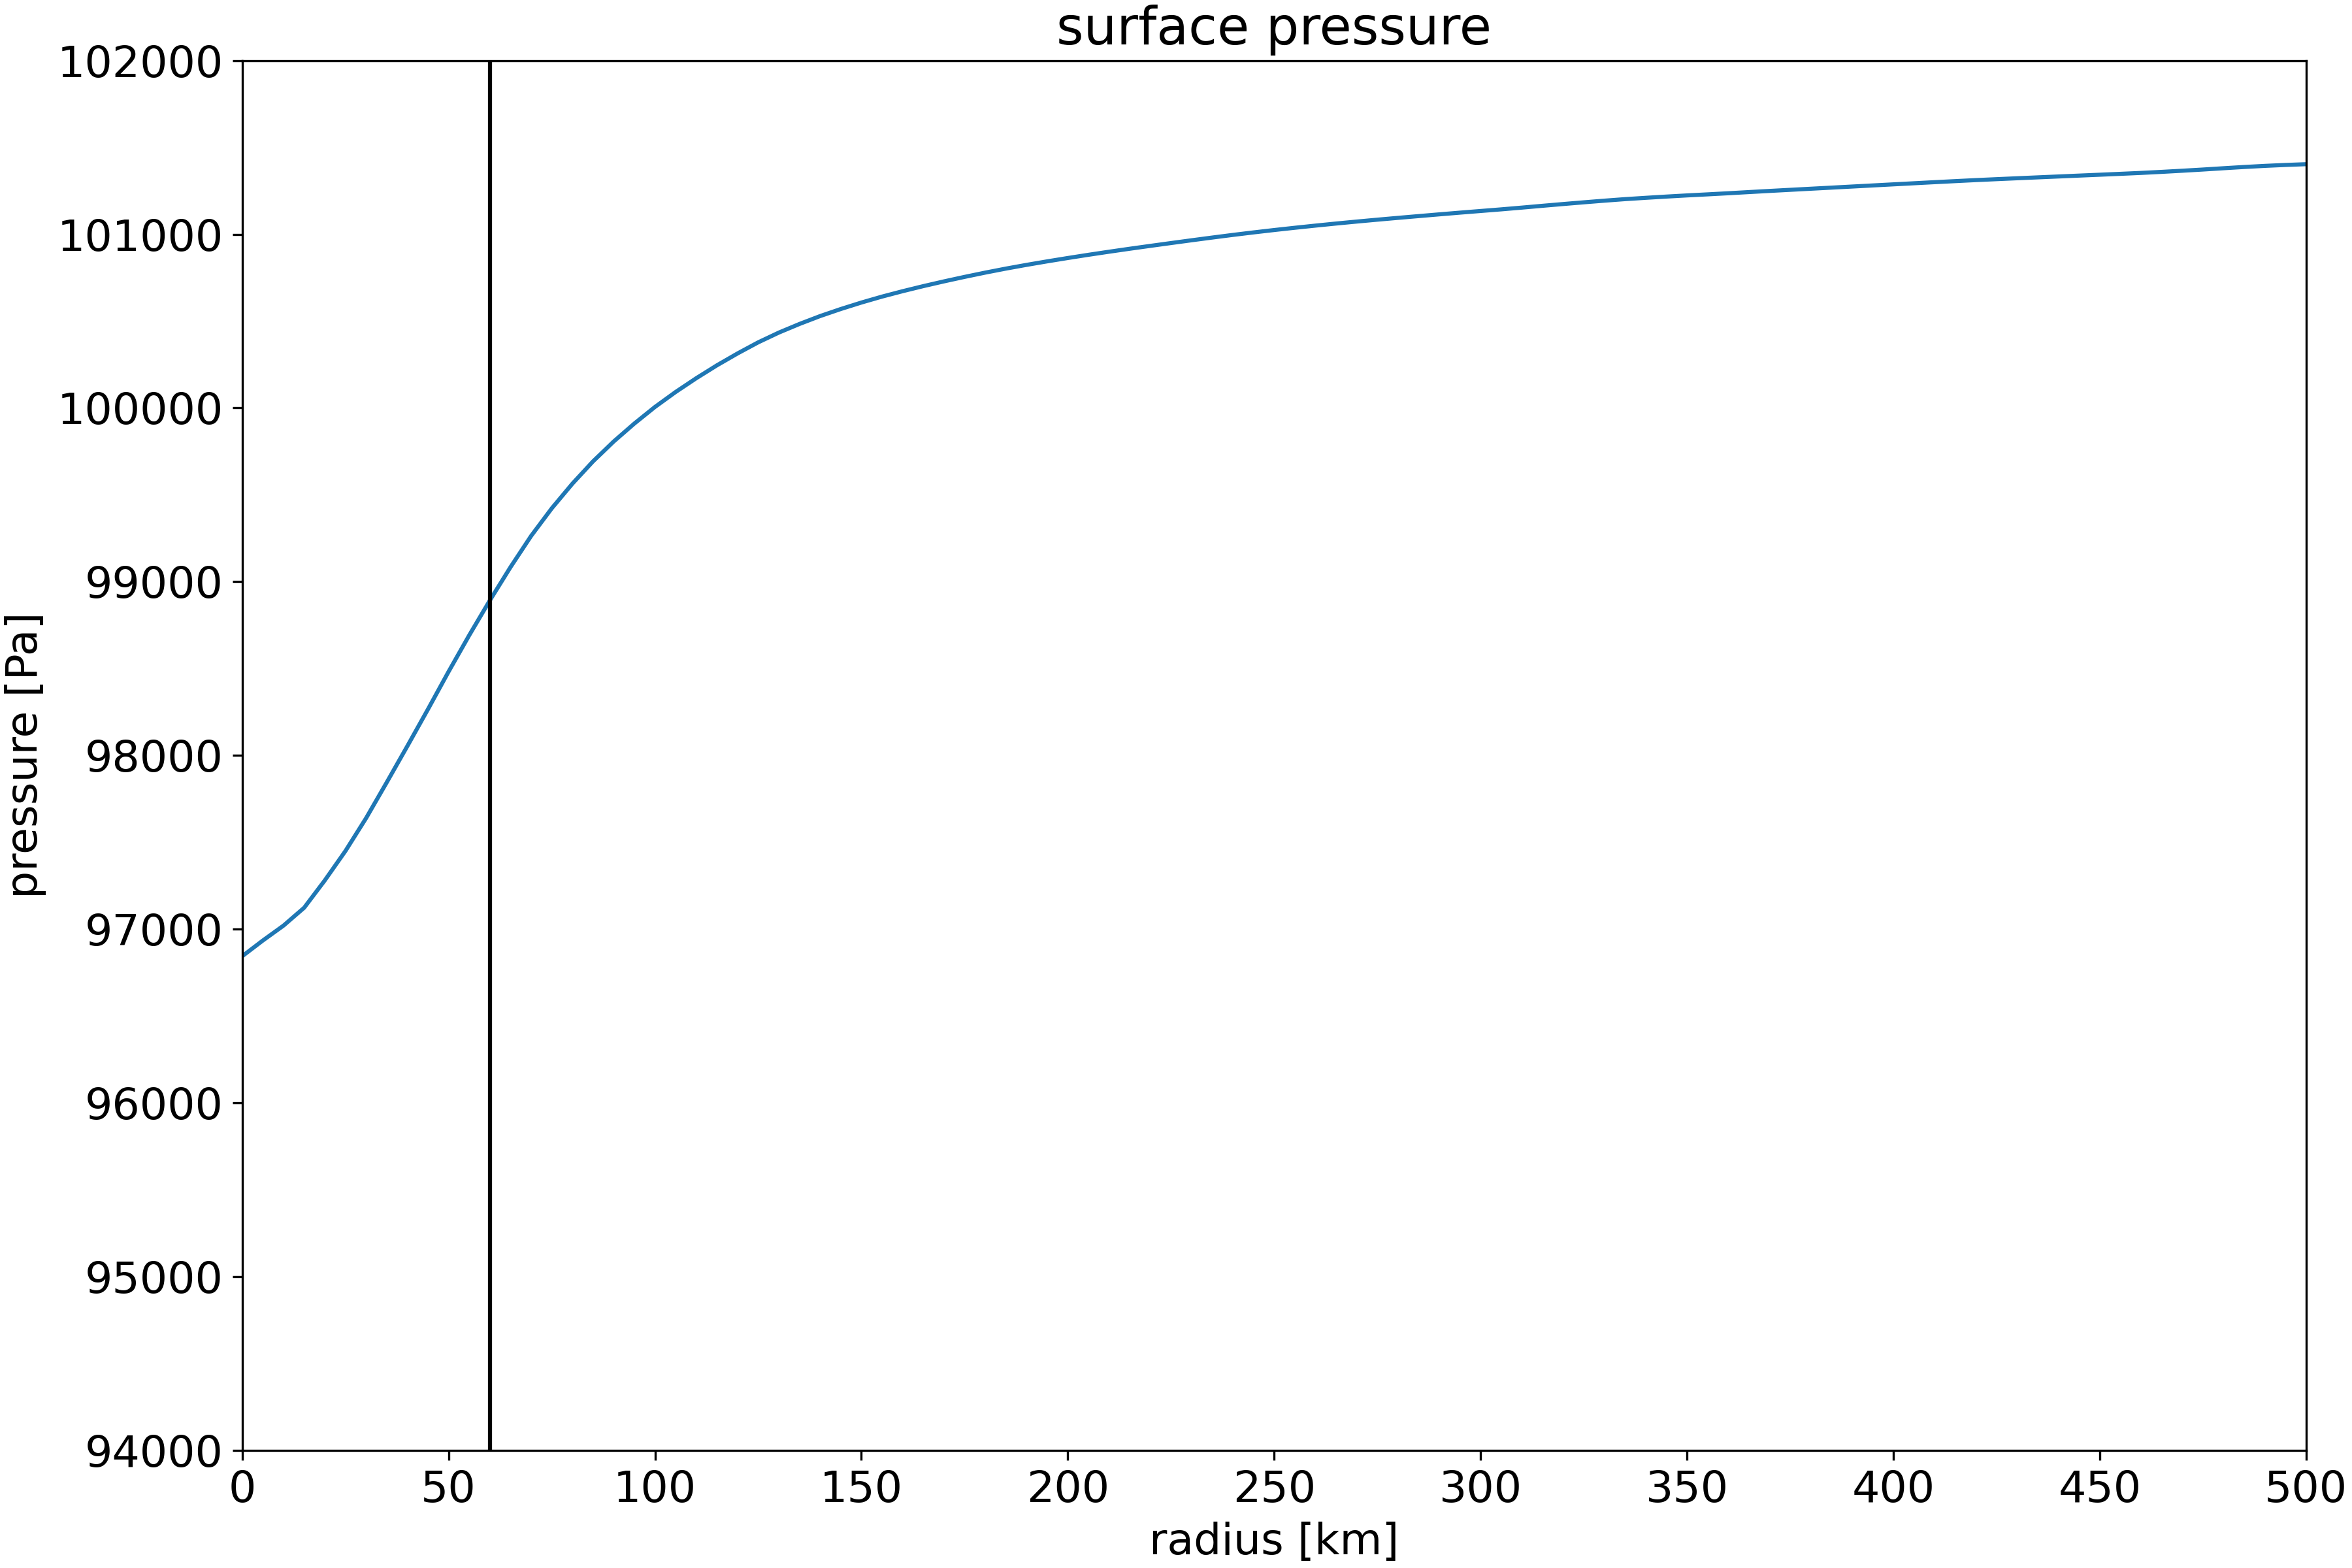
\includegraphics[width=0.85\linewidth]{img/0299554pres_msl20130905T120000Z_redo.png}
	\end{subfigure}


	\caption[short]{Azimuthal mean plots. From left to right and top to bottom: radial wind, tangential wind, vertical wind, temperature difference, vorticity and sea level pressure. The vertical black line marks the radius of maximum wind. The TC (99554) is category 4 and its track can be seen in Fig.~\ref{fig:matching_plot_cat4}.}
	\label{fig:azimean}
\end{figure}


\section{Variation of the Warm Core Criterion strength}
With the aim of understanding the impact of different warm core criteria strengths, the resulting cyclone distributions for a range of different \textbf{temdif} values were compared. As can be seen in Fig.~\ref{fig:temdif-analysis}, a weaker warm core criterion leads to a distribution with more lower-intensity storms. When comparing with the absolute counts, it can be seen that this is the result from weaker storms being tracked for lower \textbf{temdif}s. Logically, for TCs of category 2 and upwards, no difference in the counts is observed. Furthermore for \textbf{temdif}s larger than \unit[1]{K}, no tropical depressions which correspond to category -1 are tracked. It can therefore be concluded that the warm core criterion can be used very efficiently to filter out noise if only strong TCs are of interest.

\begin{figure}[!htb]
	\begin{minipage}[t]{0.48\textwidth}
		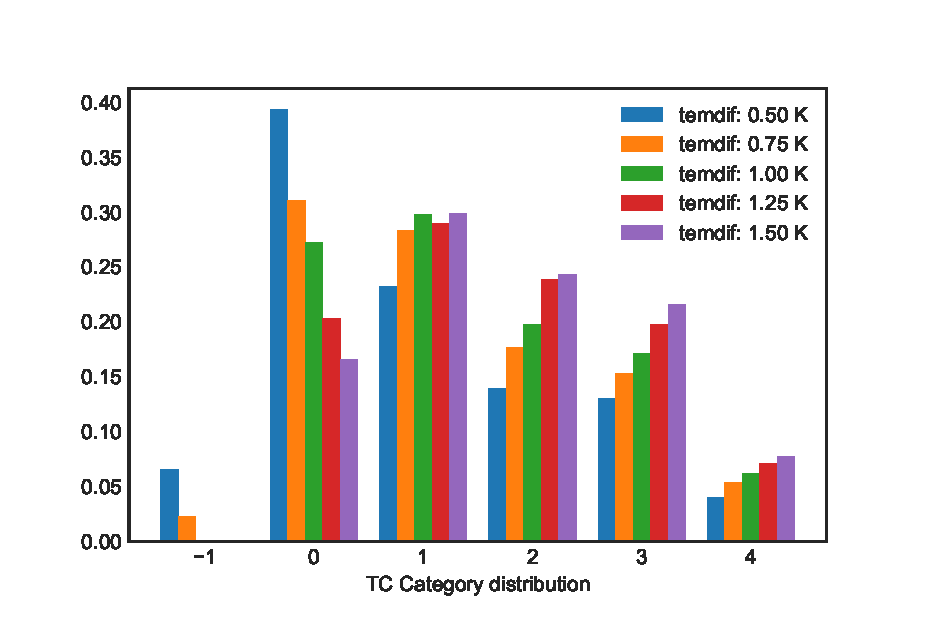
\includegraphics[width = \textwidth]{img/max_cat_distr_temdifs.eps}
	\end{minipage}
	\hfill
	\begin{minipage}[t]{0.48\textwidth}
		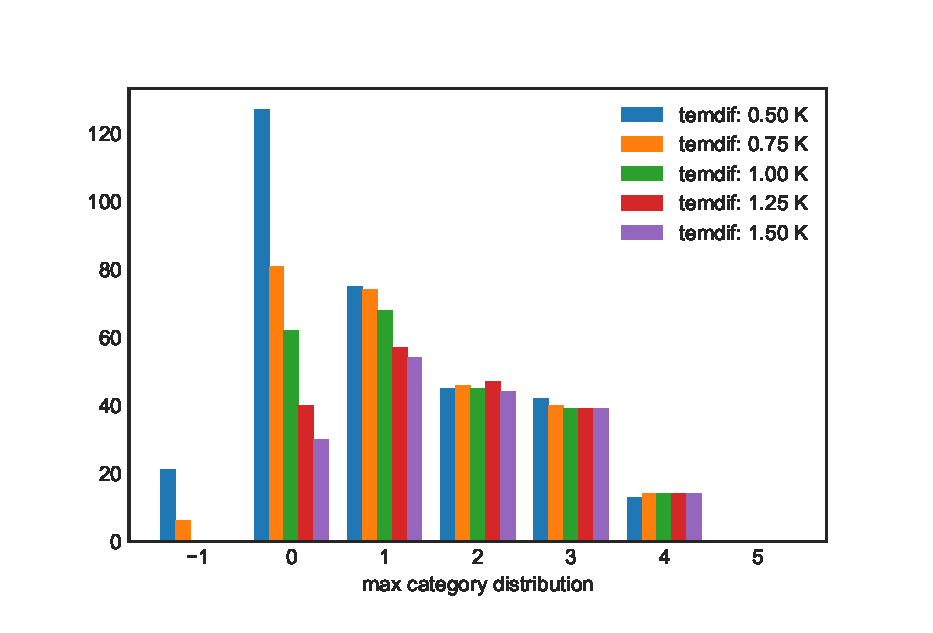
\includegraphics[width = \textwidth]{img/max_cat_counts_temdifs.eps}
	\end{minipage}
	\caption{Maximum TC category histograms for different \textbf{temdif} parameters. Each histogram on the left has unit norm. The right plot shows the absolute counts of TCs. The X-axis describes the TC categories as defined in Tab~\ref{tab:simpson-scale}. Comparing the normalised distributions on the left with the absolute counts on the right shows the good agreement of the algorithm for different values of \textbf{temdif} on strong TCs and the higher frequency of lower category storms for the lower \textbf{temdif} values.}
	\label{fig:temdif-analysis}
\end{figure}

\section{Comparison of the Warm Core Criterion and the Vorticity Threshold}\label{sec:warmcore-var}
In order to compare the importance of the warm core criterion with the vorticity threshold, only the TC tracks that were found using the parameter combinations from Tab.~\ref{tab:vor-tem-comparison} were analysed. These combinations were chosen because they correspond to different relative strengths of the two criteria.

\begin{table}[!htb]
	\centering
	\begin{tabular}{|l|l|l|}
		\hline
		\textbf{parameter} & \textbf{unit} & \textbf{values}  \\ \hline
		slpdis             & m             & 100000           \\
		vormin             & 1/s           & 1e-6, 1e-5, 1e-4 \\
		temdif             & K             & 0.5, 1 ,1.5      \\
		temdis             & m             & 200000           \\ \hline
	\end{tabular}
	\caption{Parameter combinations used for the comparison}
	\label{tab:vor-tem-comparison}
\end{table}

It was expected that the vorticity threshold should influence the distribution of tracked TCs only if a weak warm core criterion is applied. This was hypothesised because most low pressure systems with strong warm cores should exhibit the necessary minimum vorticity while weak warm core systems might not have a strong enough rotating motion. However, as can be seen in Fig.~\ref{fig:temdif-vormin-comp}, even with a very weak warm core criterion does the vorticity threshold not influence the storm intensity distributions. A comparison for different values of \textbf{temdif} and an analysis of the impact of the vorticity criterion on the storm lifetime can be found in the Appendix.
\begin{figure}[!htb]
	\centering
	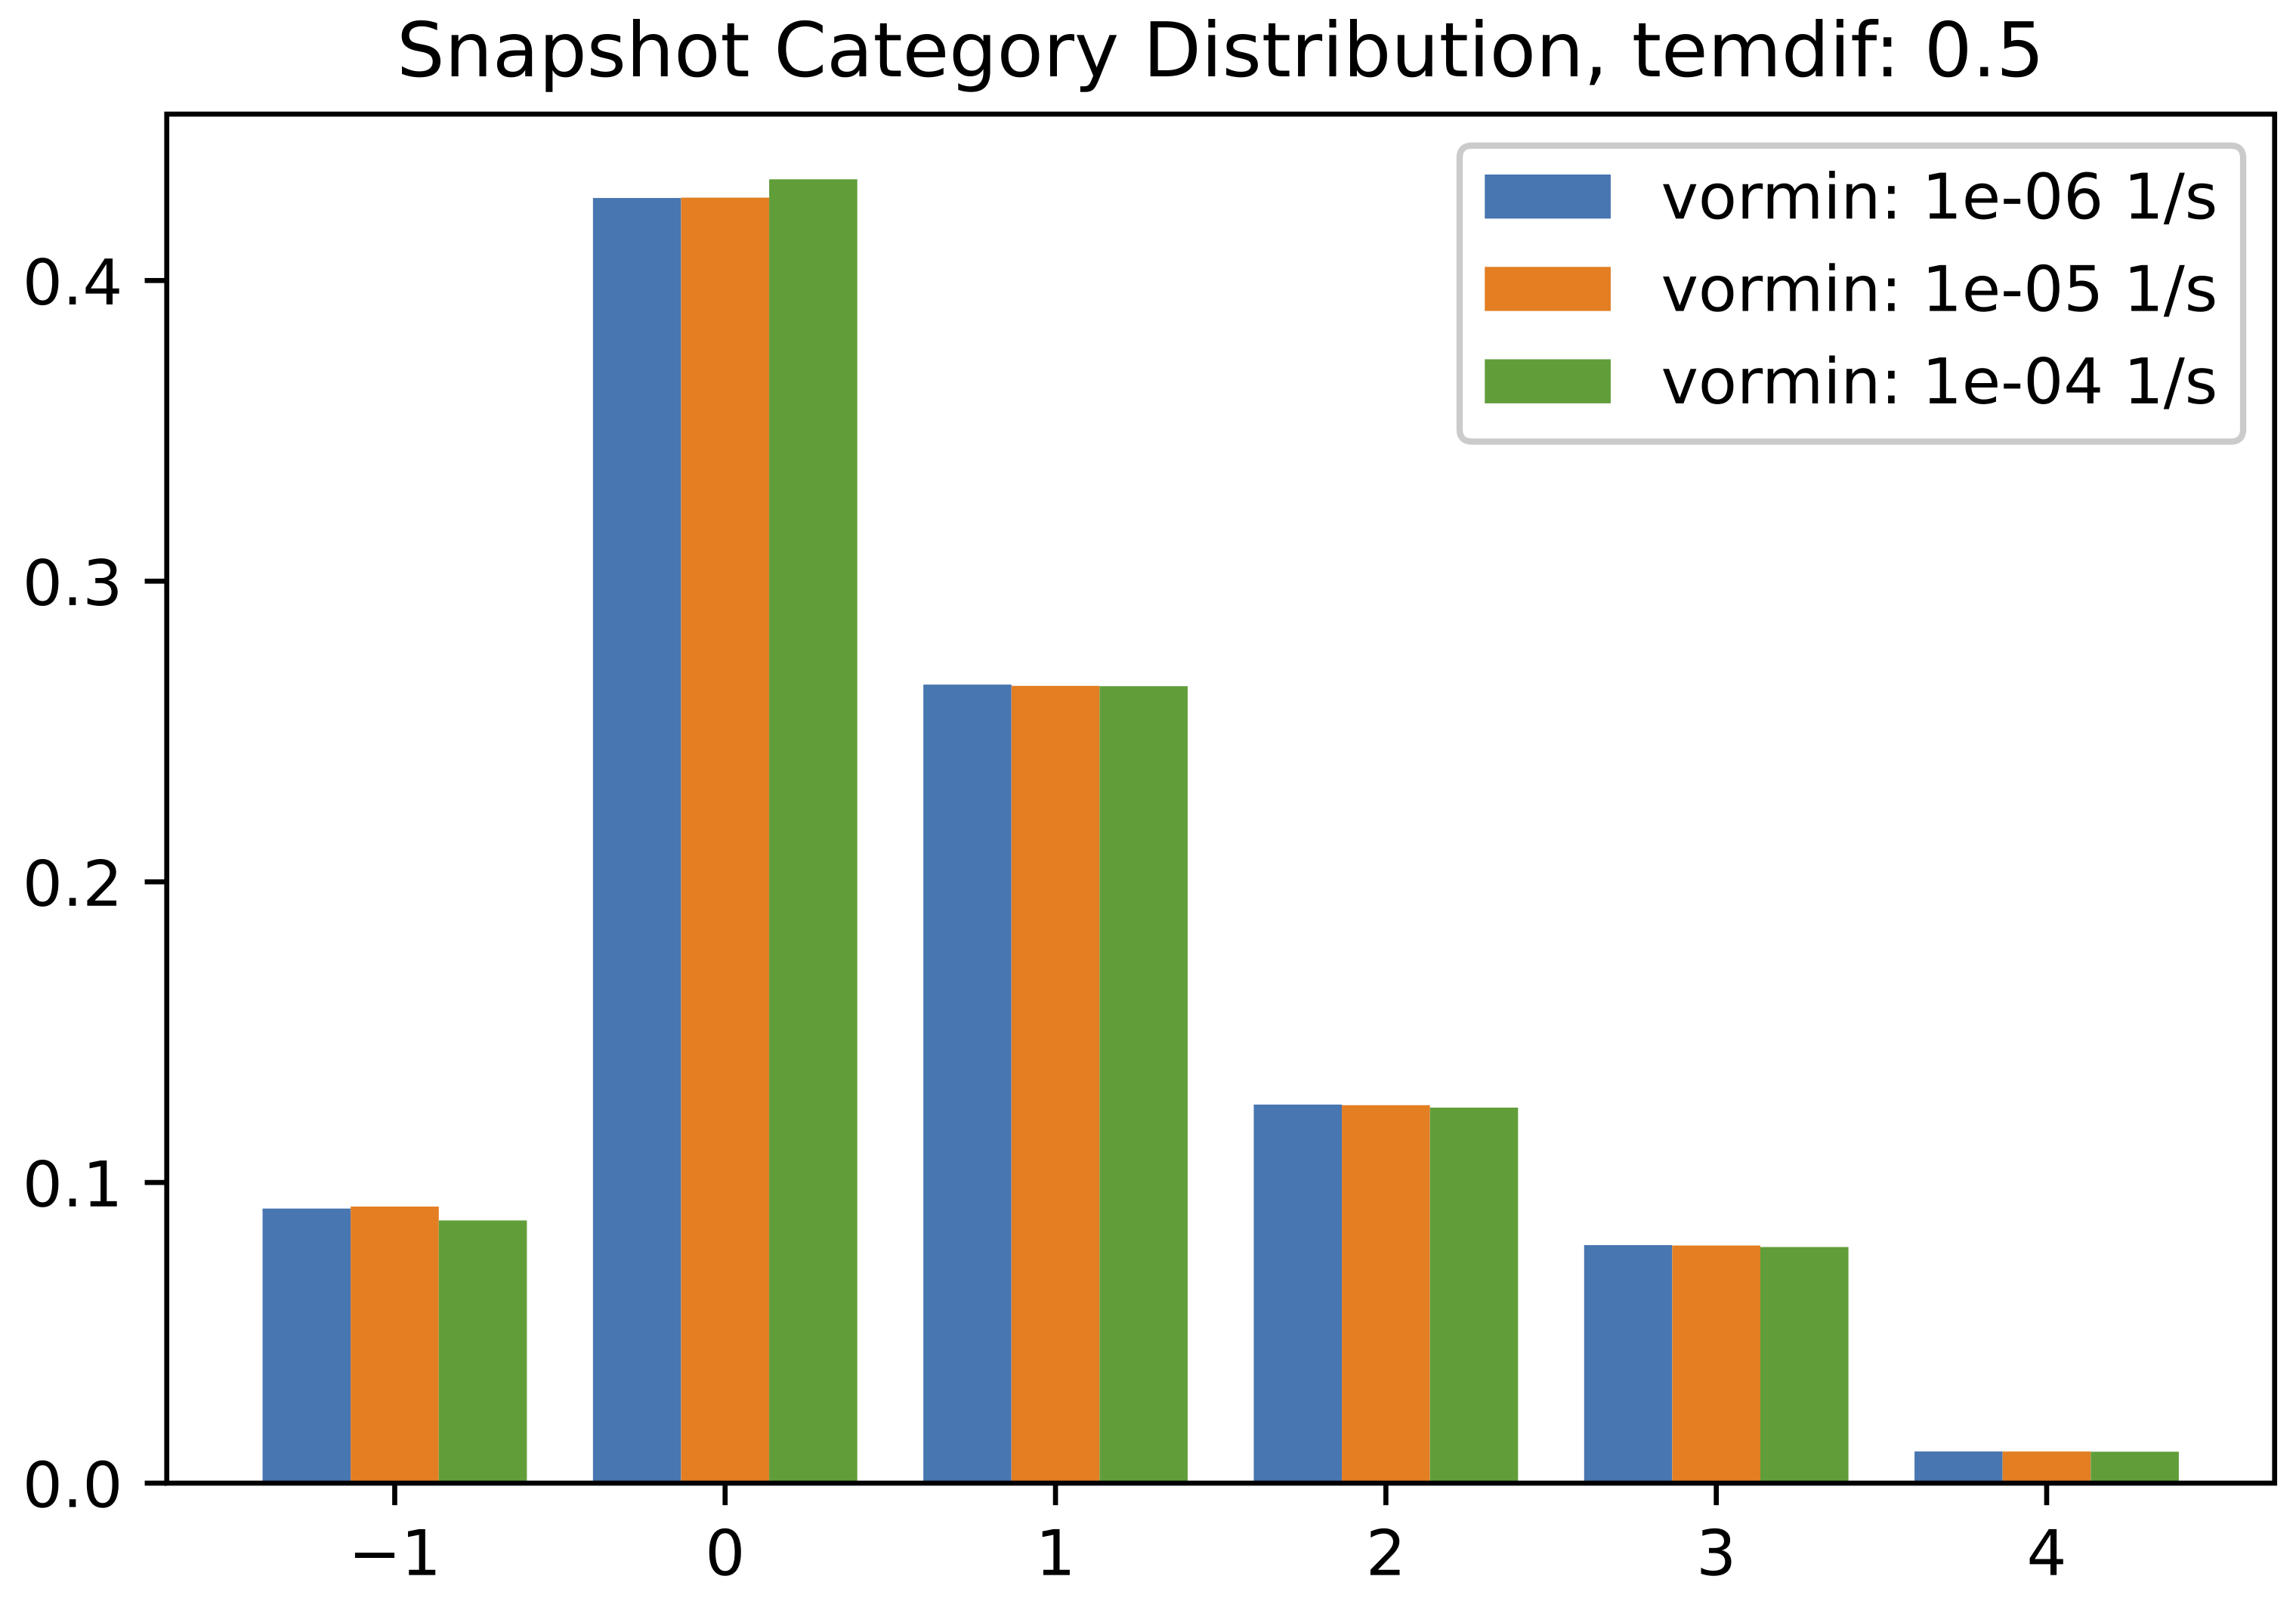
\includegraphics[width=0.5\textwidth]{img/curr_category_vortem05.png}
	\caption{Snapshot category distribution for a weak warm core criterion and several vorticity thresholds. The Y-axis shows the normalised counts.}
	\label{fig:temdif-vormin-comp}
\end{figure}

\section{TC Genesis regions}
A direct consequence of the observations from Sec.~\ref{sec:warmcore-var} is that with a weaker warm core criterion the TCs can be found already when they have not had much time to intensify. This is relevant because from best track data it is expected that most TCs form in the main development region (MDR) which lies roughly between 10 -- 20 \degree N and 20 -- 80 \degree W. However, when checking the genesis locations and density in Fig.~\ref{fig:genesis-temdif1}, it can be seen that the formation of TCs in ICON is not limited to the MDR. When using a weaker warm core criterion, the areas of highest TC density shift more towards the expected region. This can be interpreted as the successful detection of TCs in earlier development phases.
\begin{figure}[!htb]
	\centering
	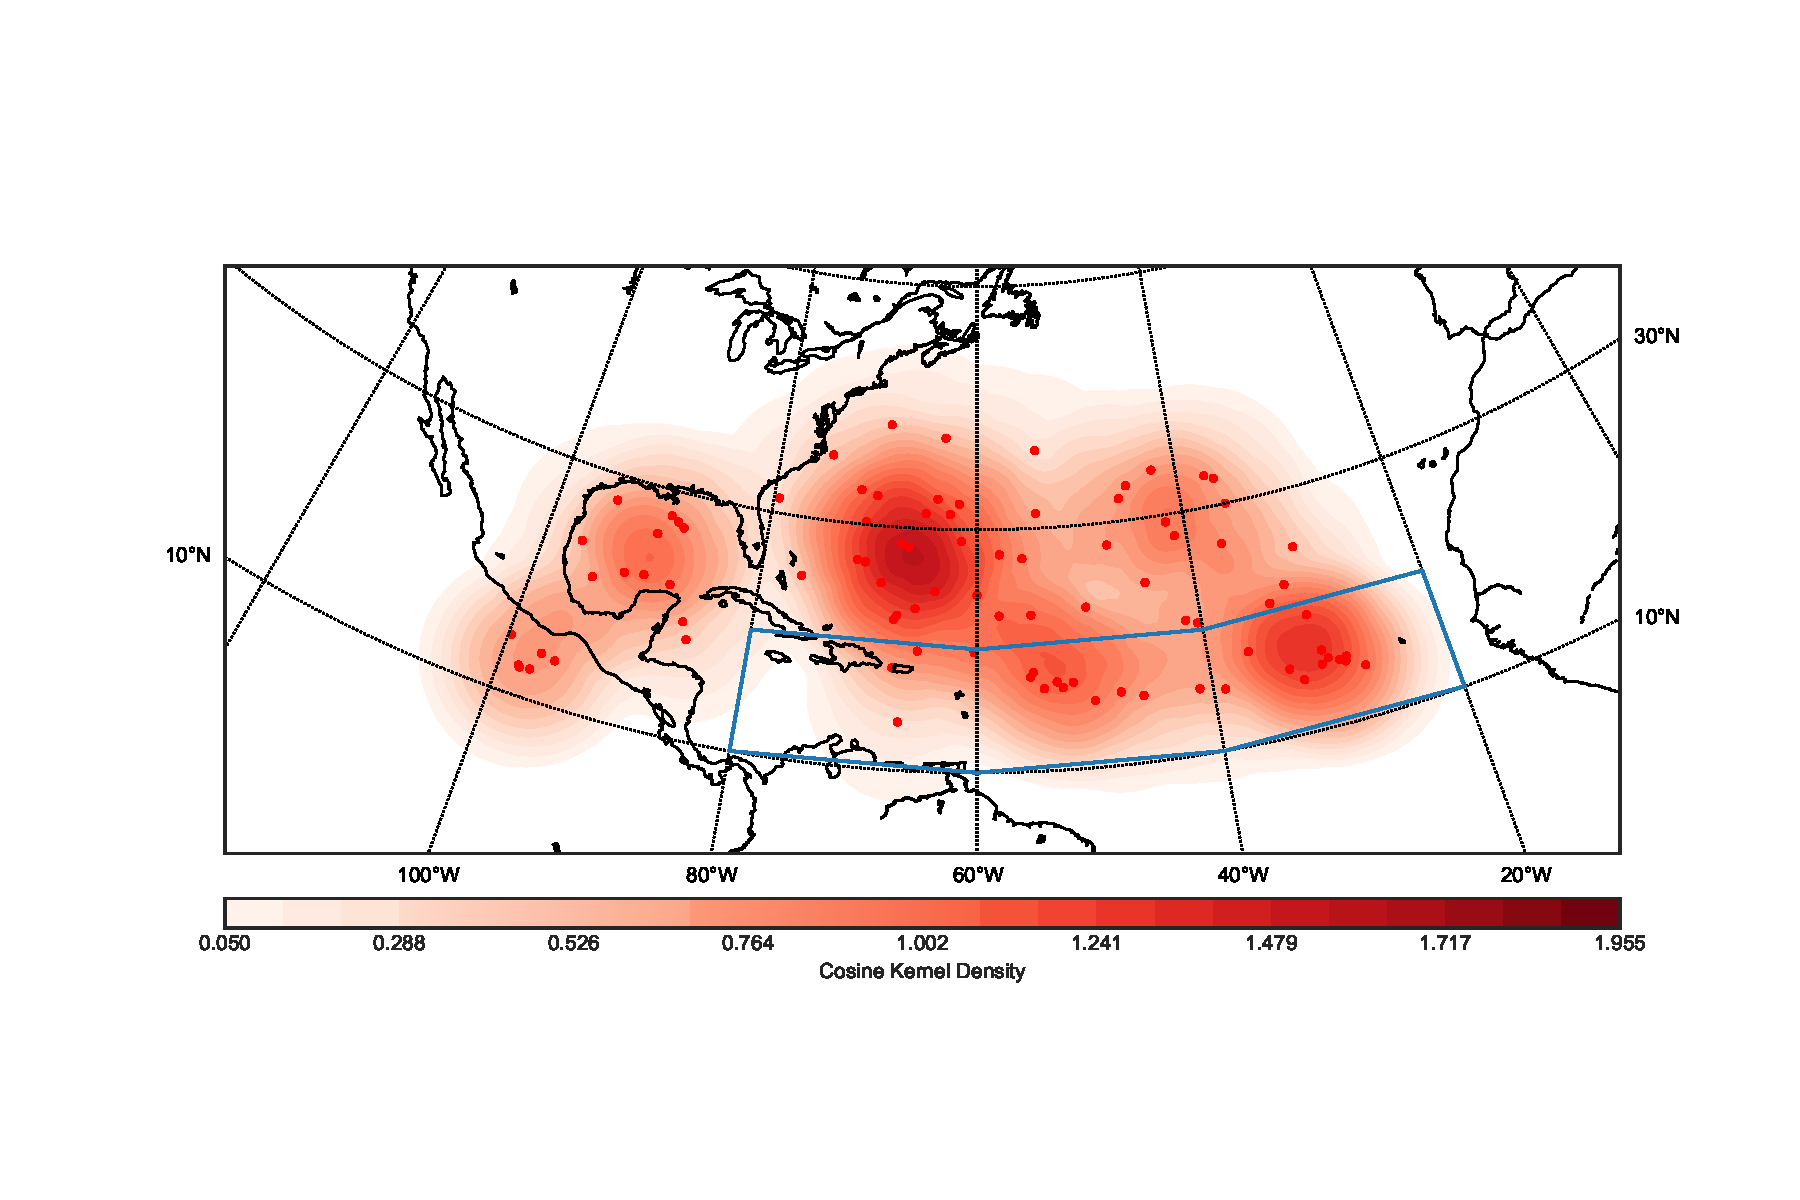
\includegraphics[width=0.7\textwidth]{img/genesis_plot_temdif1.pdf}
	\caption{Genesis spots and density for temdif = 1.0. Using param\_id = 149.}
	\label{fig:genesis-temdif1}
\end{figure}

\section{Track occurrence frequency }
It has been shown that the choice of parameters affects typical distributions like the lifetime and intensity of the found TCs. With the purpose of assessing the effect of different warm core criteria on the length of the tracks, the point occurrence frequency was visualised. This quantity is the frequency of a specific location at a certain time being recognised as part of a TC track. Specifically, it evaluates to 1 if all parameter combinations determine a point to be a TC and to 0.5 if only half of them do. The tracks shown in Fig.~\ref{fig:occ-prob} are determined using the parameter combinations from Tab.~\ref{tab:occ-prob-params}.

\begin{table}[ht]
	\centering
	\begin{tabular}{|l|l|l|}
		\hline
		\textbf{parameter} & \textbf{unit} & \textbf{values} \\ \hline
		temdif             & K             & 0.5, 1 ,1.5     \\
		temdis             & m             & 200000          \\
		slpdis             & m             & 100000          \\
		vormin             & 1/s           & $10^{-5}$
		\\
		\hline
	\end{tabular}
	\caption{Parameter combinations used for occurrence frequency plots in Fig.~\ref{fig:occ-prob}.}
	\label{tab:occ-prob-params}
\end{table}
It can be observed that the weaker warm core criterion tracks TCs that are found by only a small part of the parameter combinations. Furthermore, the ends of TC tracks that are found in all of the three plots are longer for the lower values of temdif. Therefore, the weaker warm core criterion enables tracking in earlier development phases. This observation will be made more precise in the following section.
\begin{figure}[!htb]
	\centering
	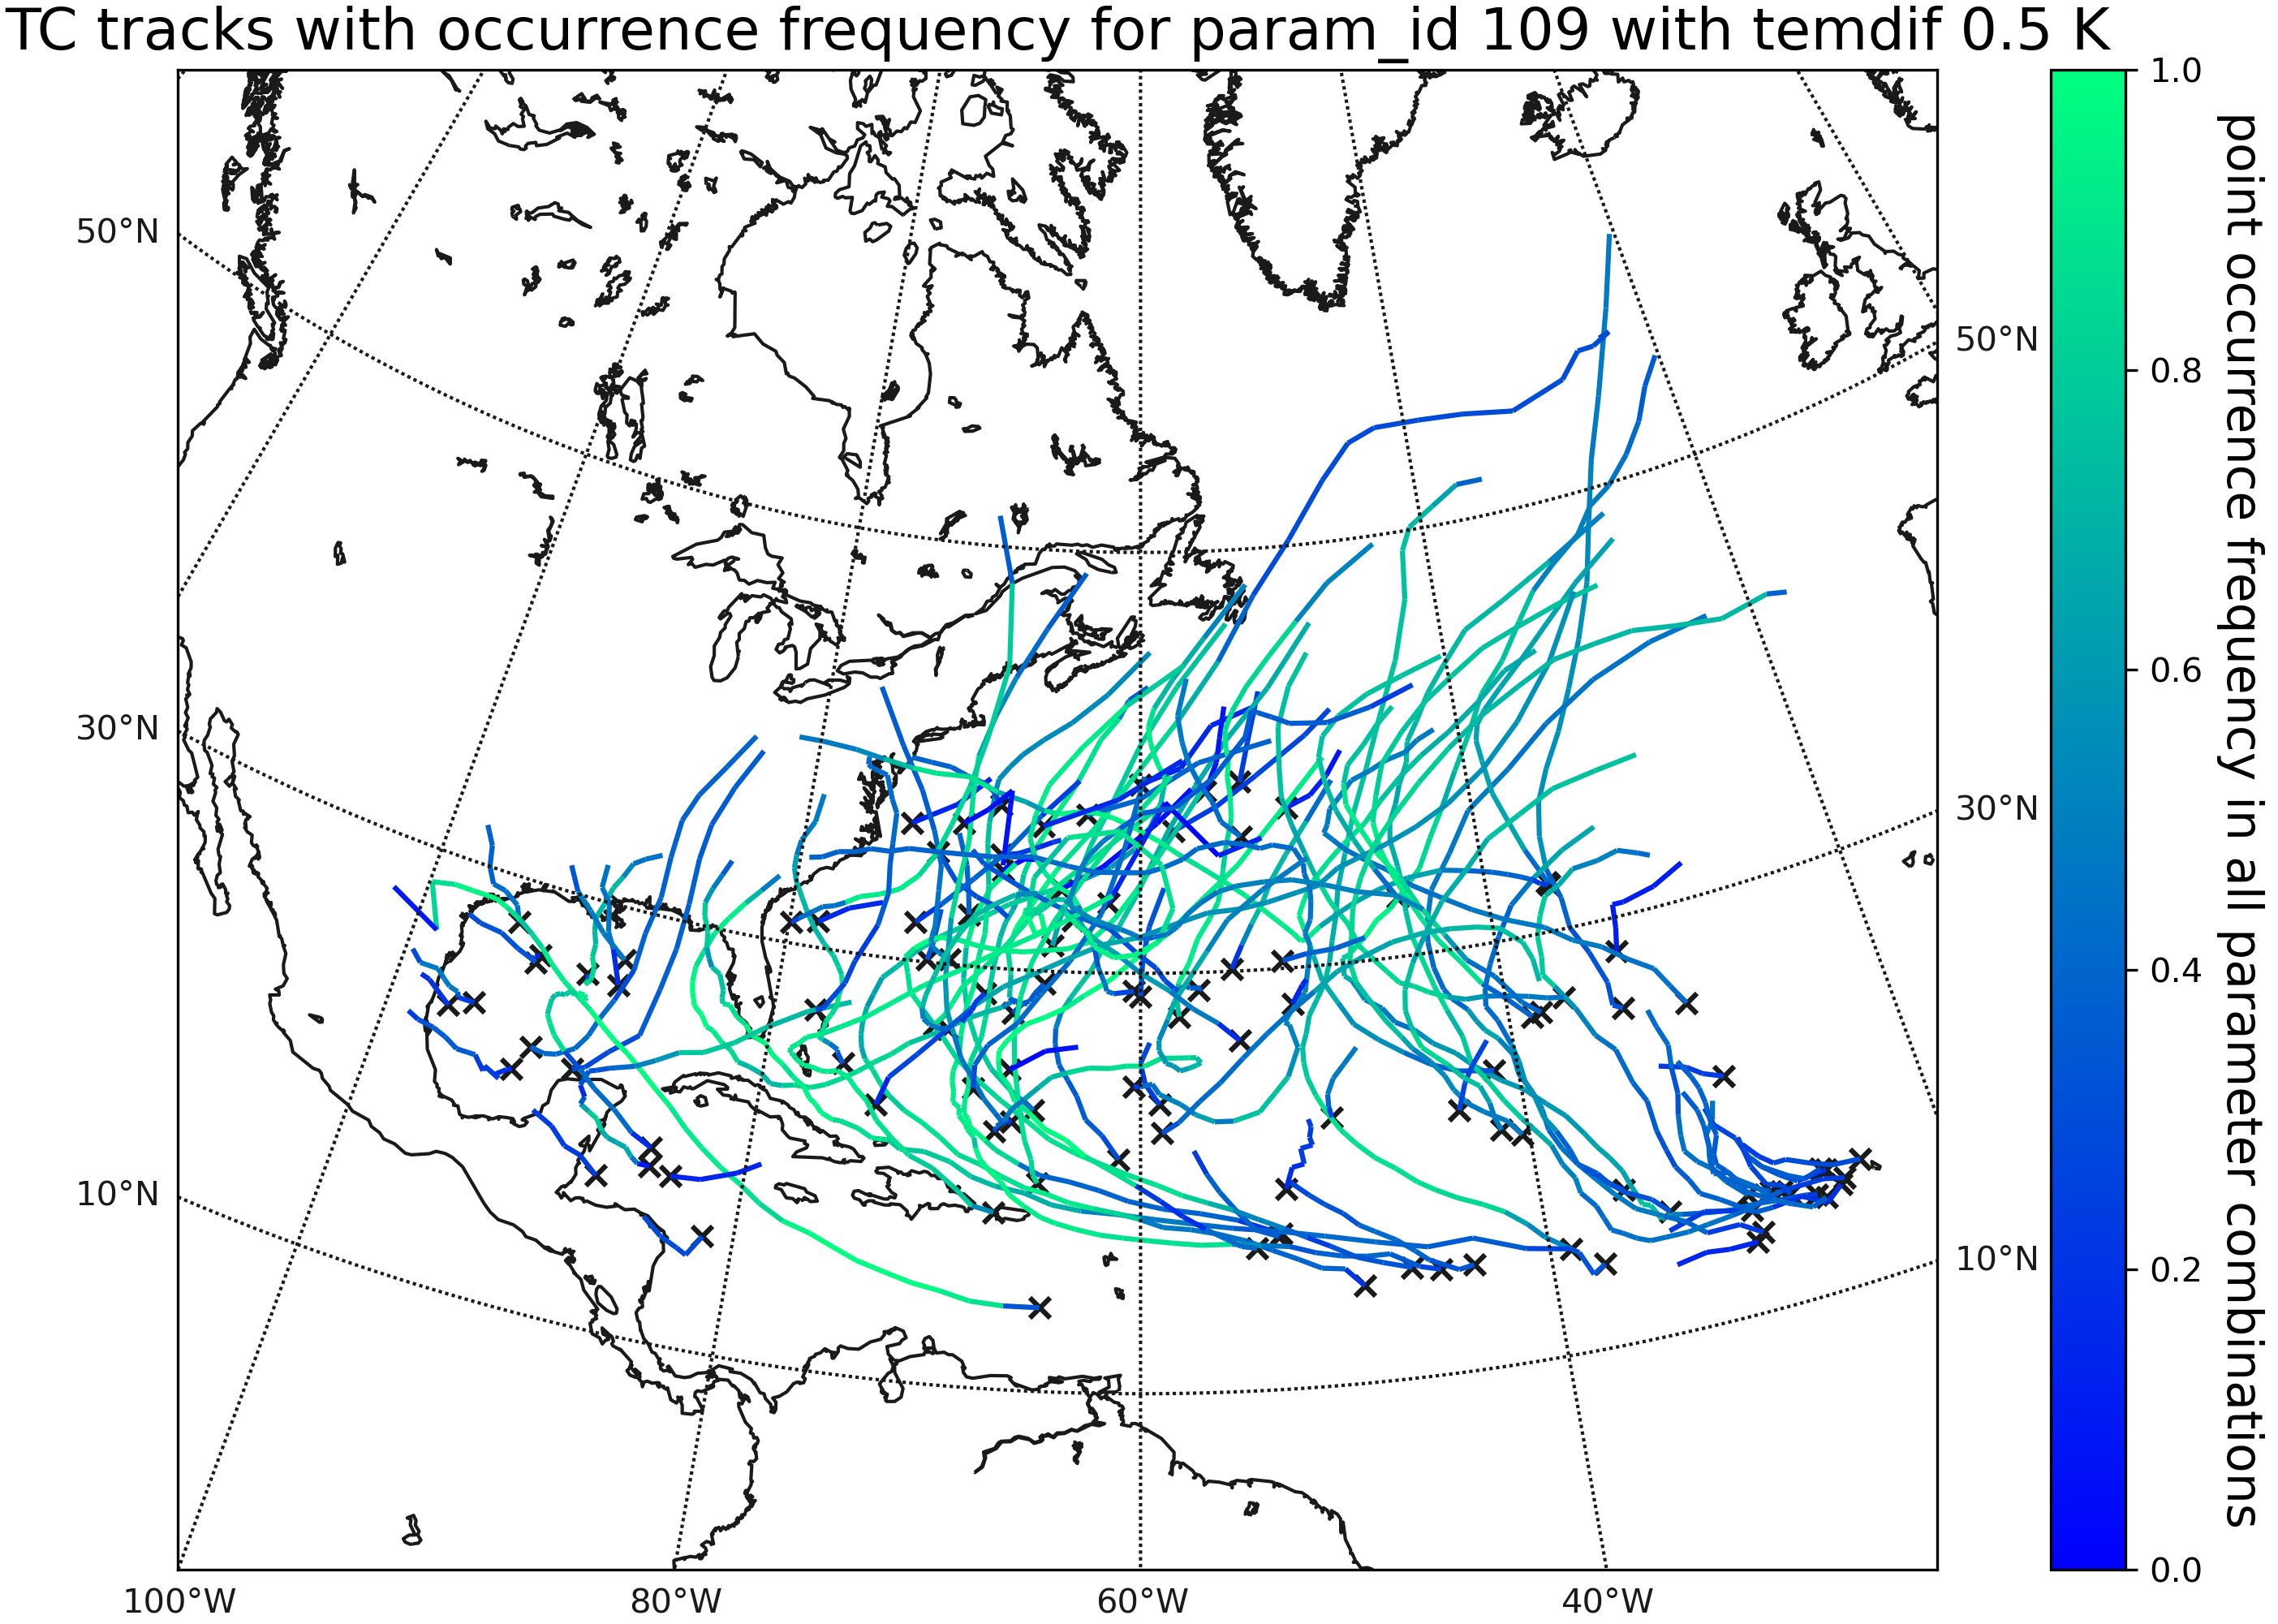
\includegraphics[width=0.6\textwidth]{img/tc_tracks_occ_prob_pid_109_temdif_05.png}
	\\[\smallskipamount]
	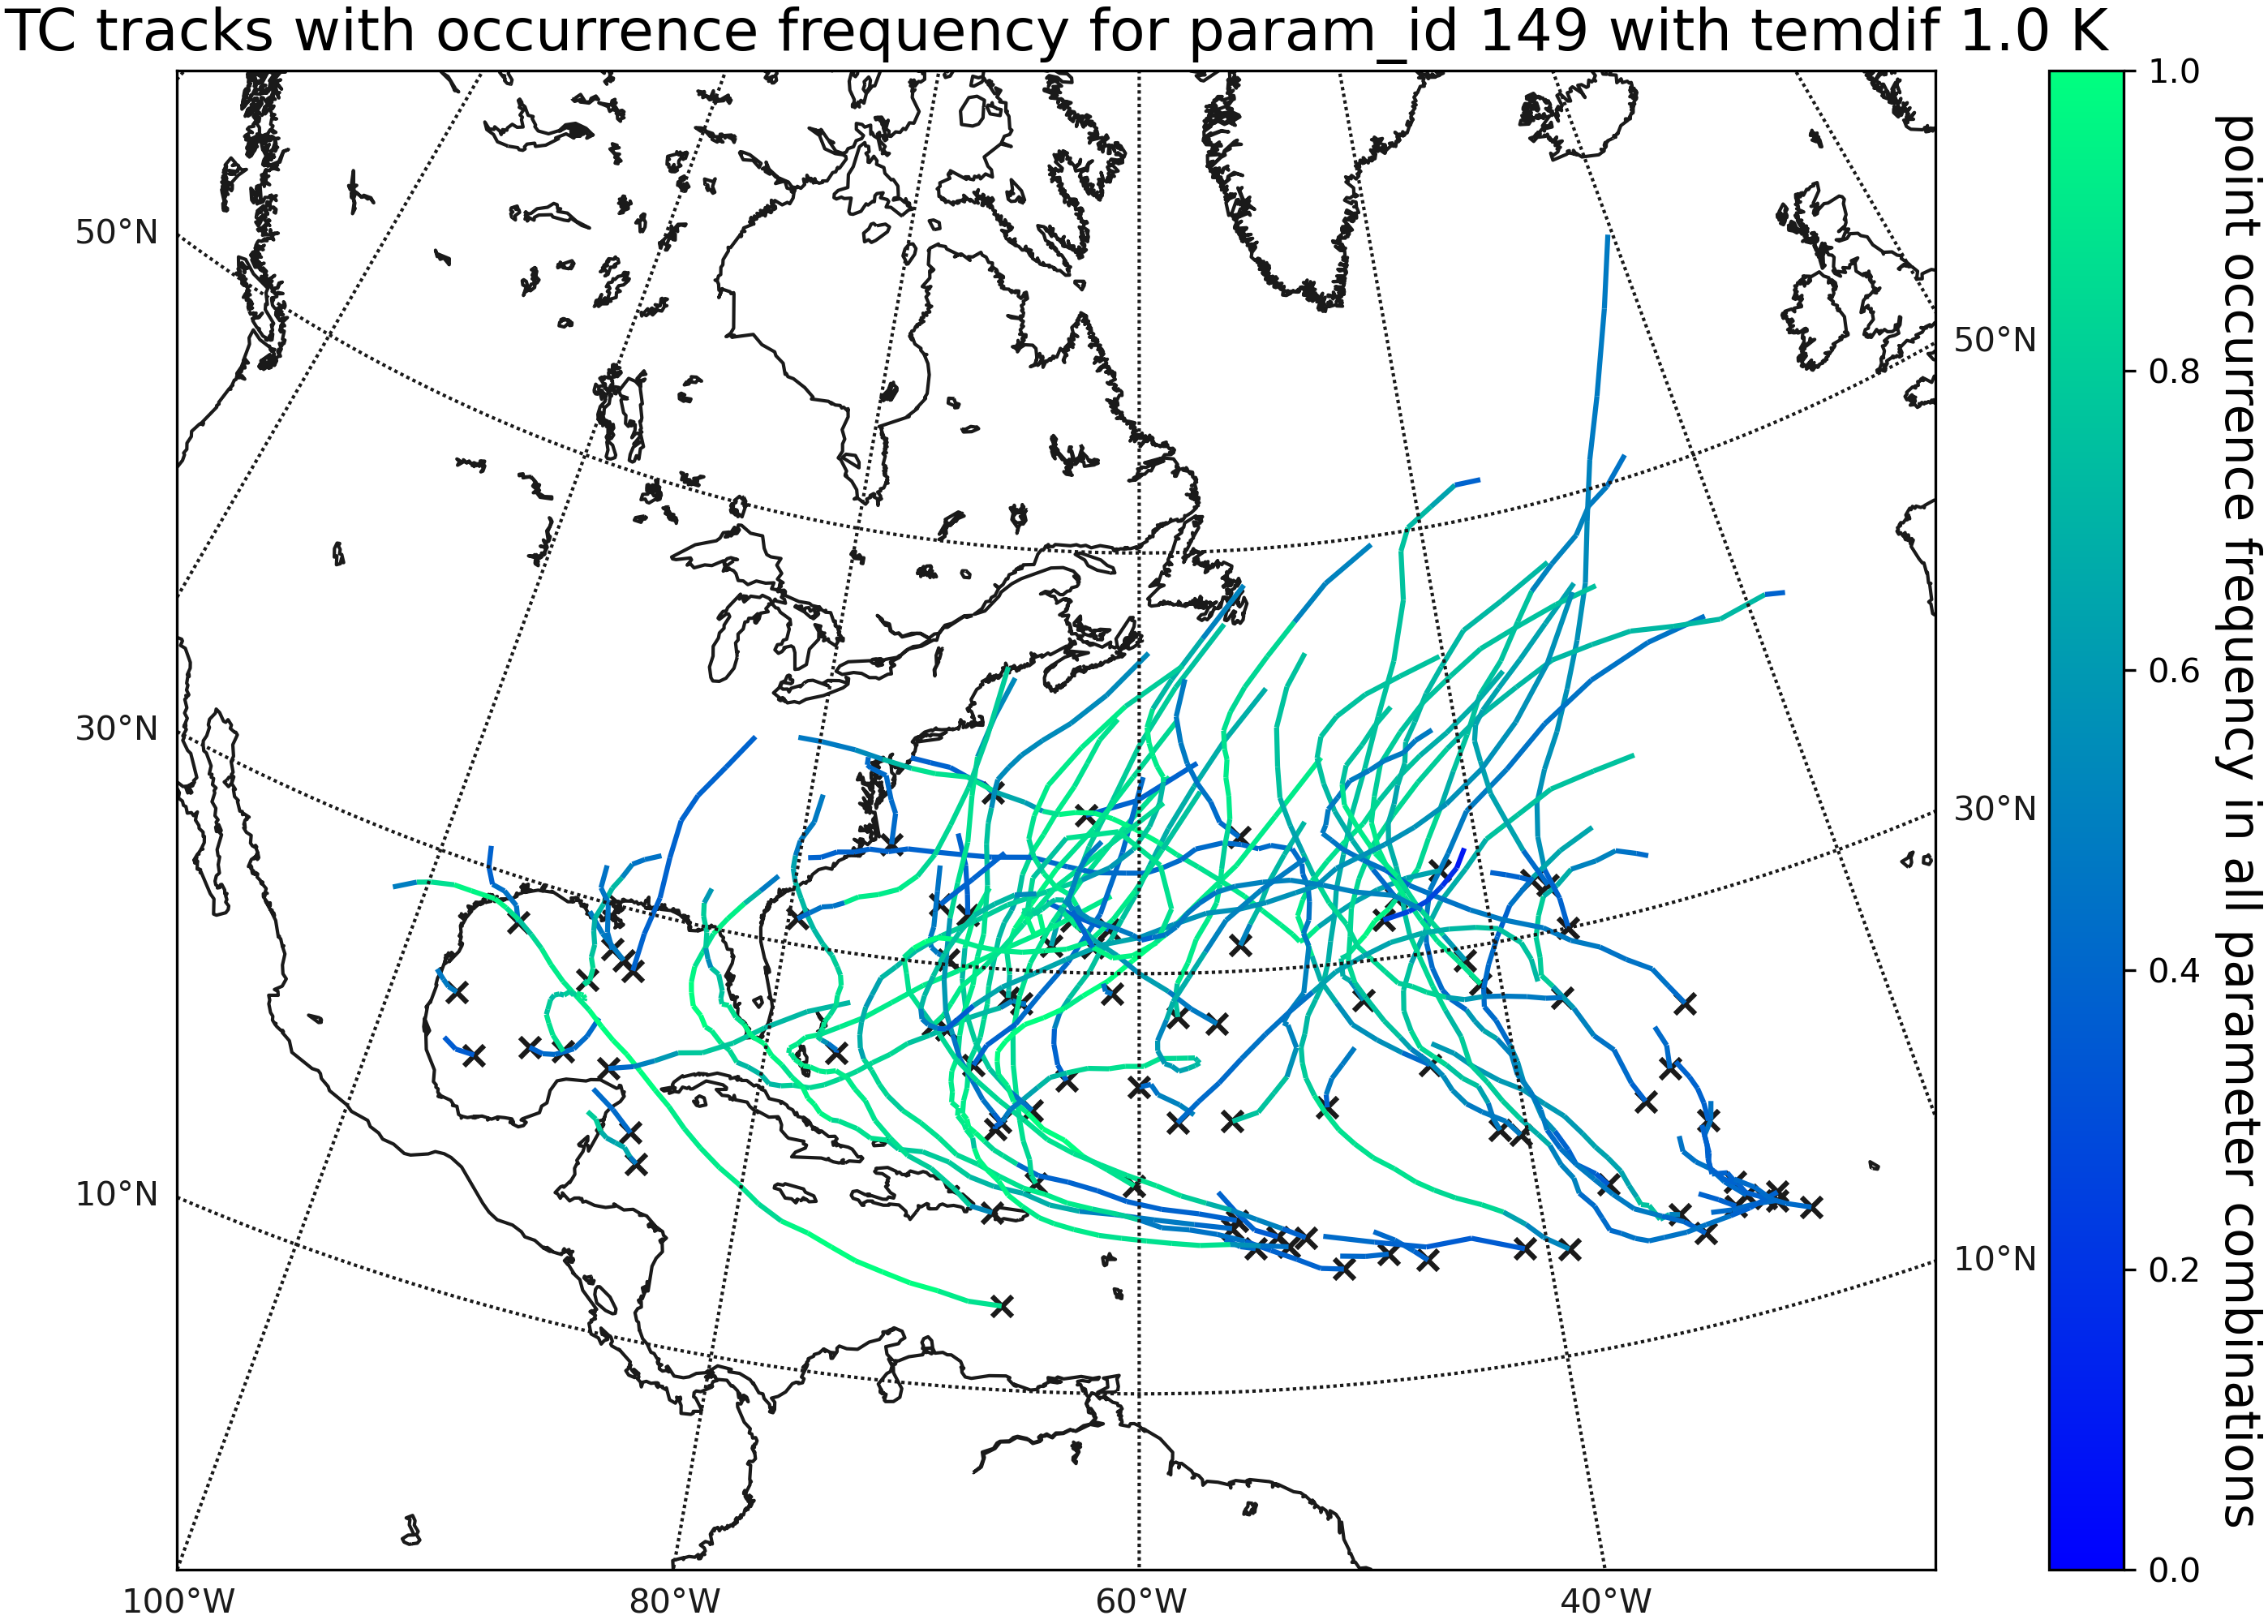
\includegraphics[width=0.6\textwidth]{img/tc_tracks_occ_prob_pid_149_temdif_10.png}
	\\[\smallskipamount]
	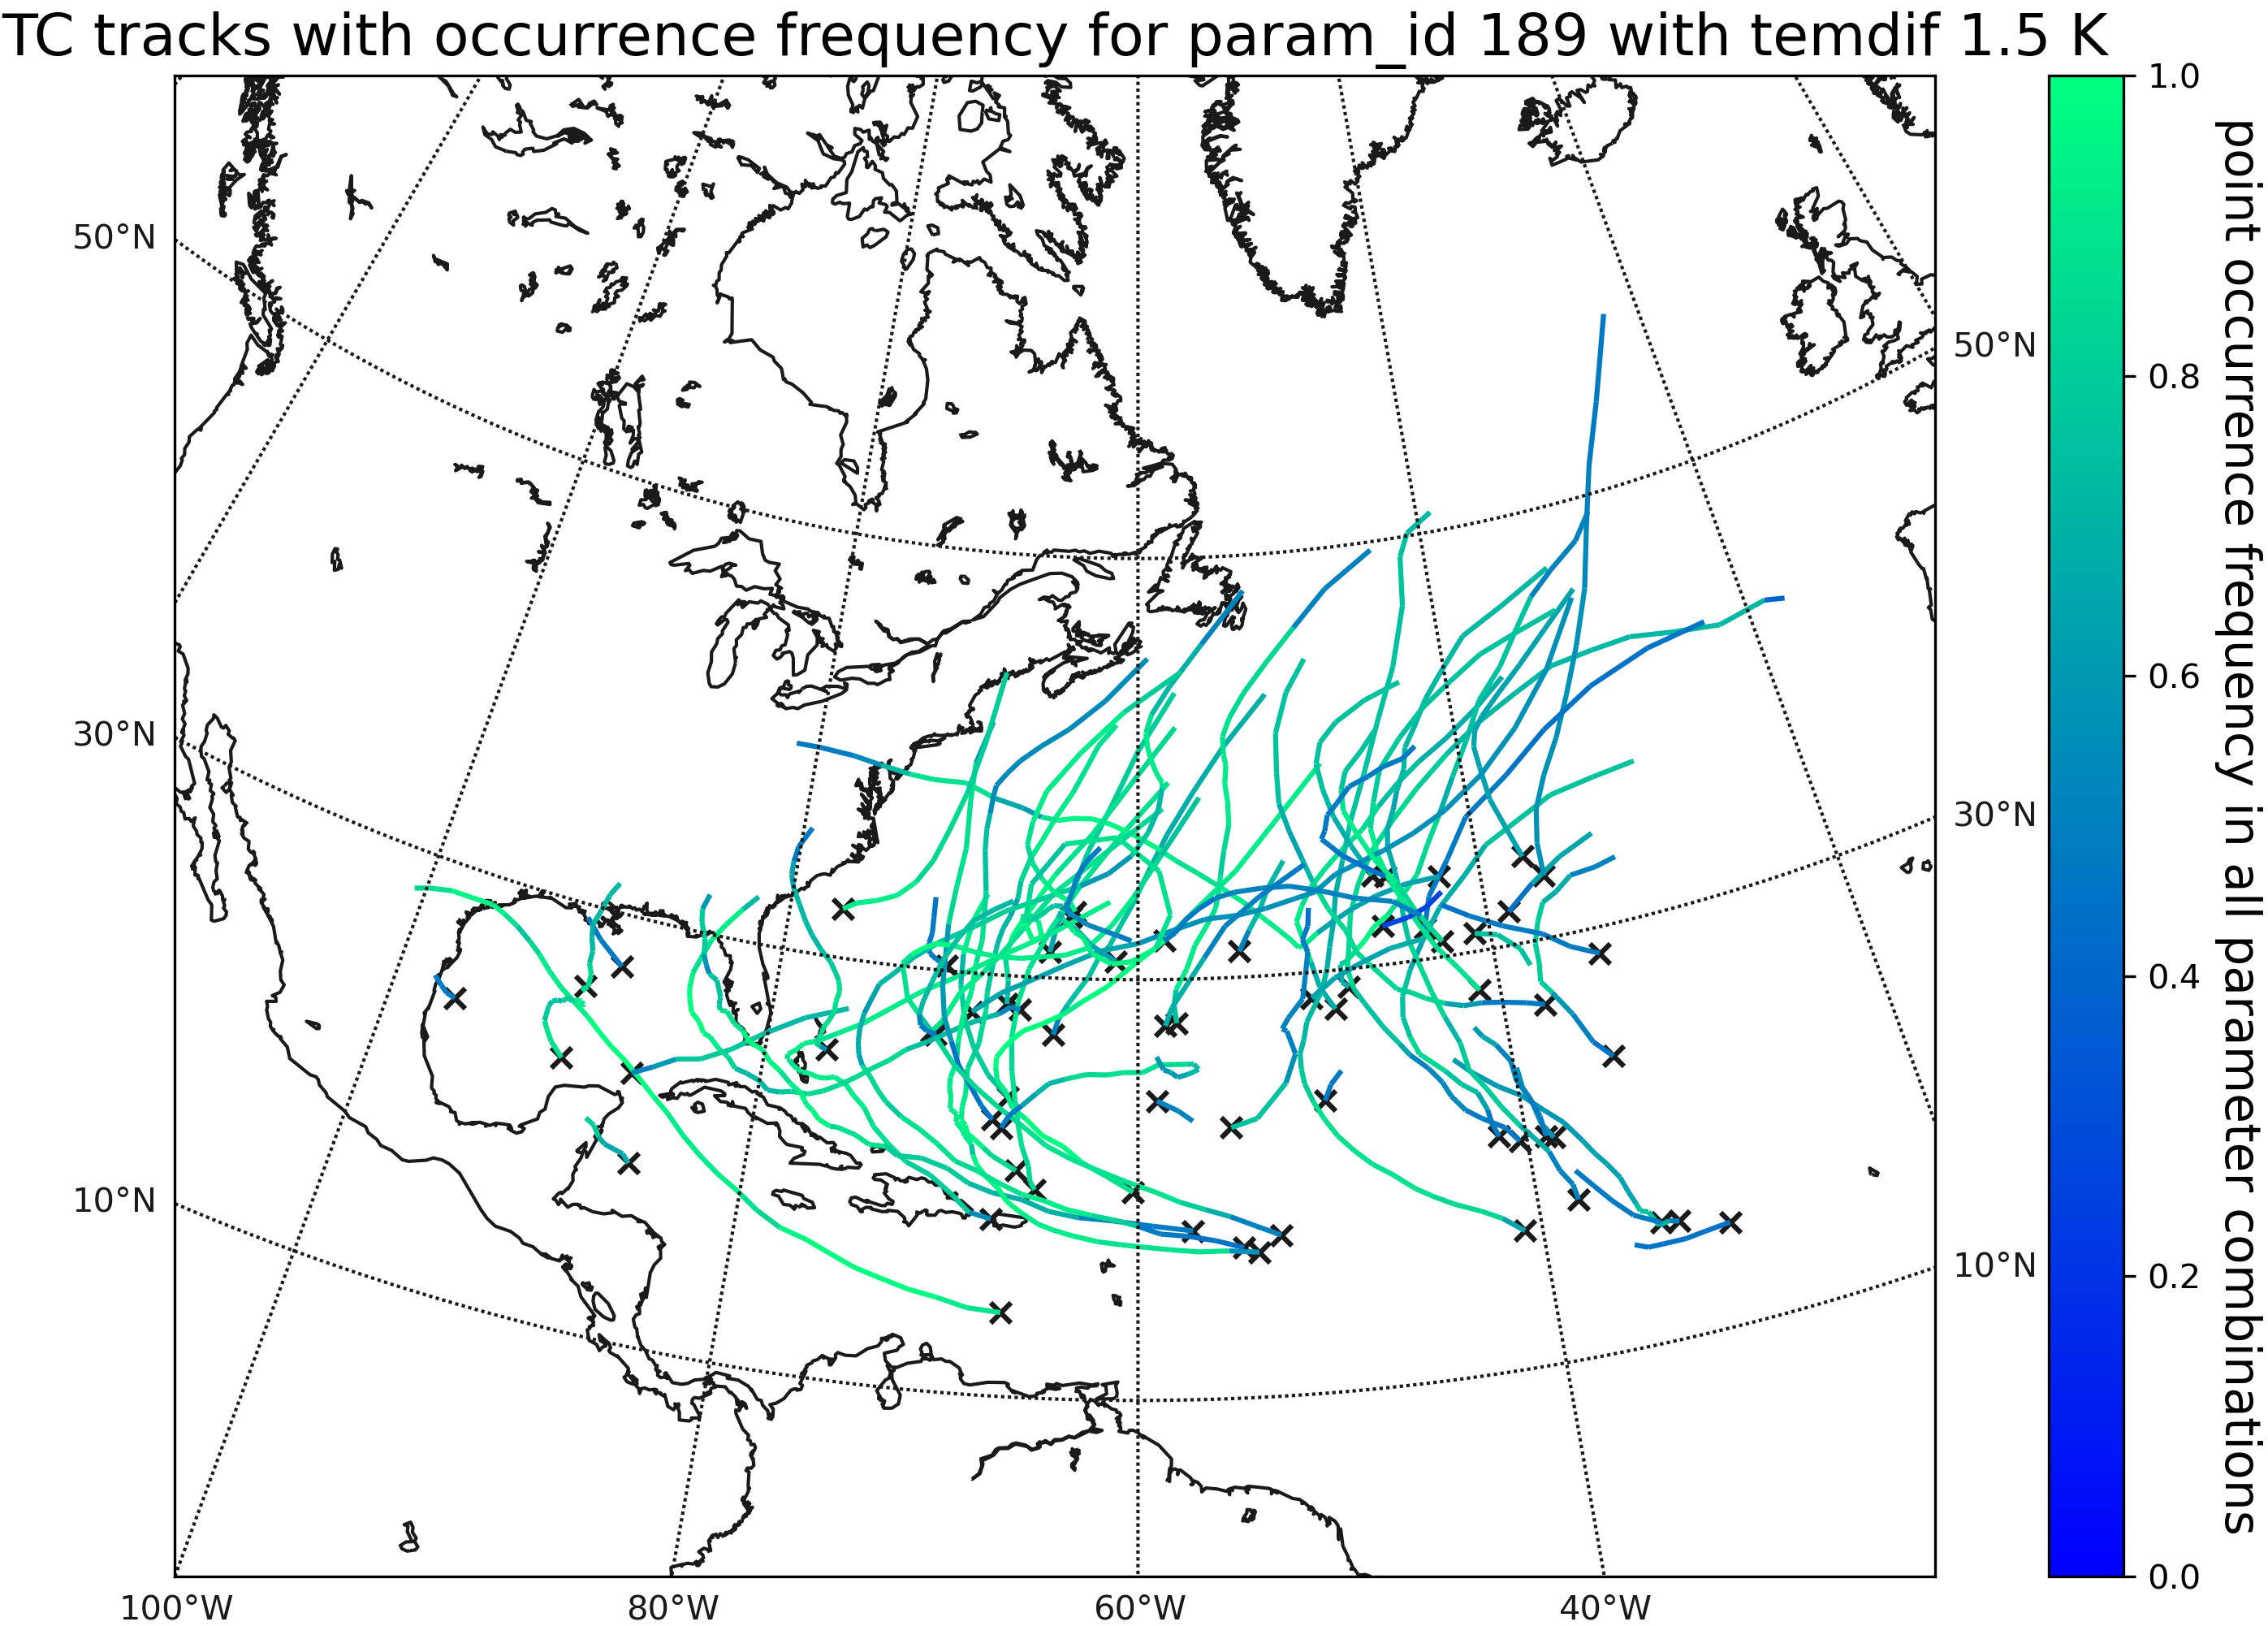
\includegraphics[width=0.6\textwidth]{img/tc_tracks_occ_prob_pid_189_temdif_15.png}
	\caption{Tracks from all ensemble members for the parameter combinations in Tab.~\ref{tab:occ-prob-params}.}
	\label{fig:occ-prob}
\end{figure}

\section{Matching TC tracks across parameter combinations}
So far the effects of different parameter variations have ben thoroughly analysed. However, it still remains to be seen if different parameter combinations identify the same TCs. In order to achieve this, different tracks were matched according to the following procedure:
\begin{itemize}
  \item choose the track of a certain TC as a base track
  \item find the point of maximum wind of this track
  \item match tracks found in the same simulation run created with different parameter combinations if: they have an entry at the same time like the maximum wind entry of the base track and at a position within \unit[70]{km}
\end{itemize}
Finally, all tracks, their start- and end-points, the TC intensity and the occurrence frequency within the family of tracks were plotted. This analysis was performed on 100 tracks sampled from all parameter combinations and for 58 tracks that were found using the original parameter combination. A resulting plot from the first selection can be seen in Fig.~\ref{fig:matching_plot_cat4}.\newline
\begin{figure}[!htb]
	\centering
	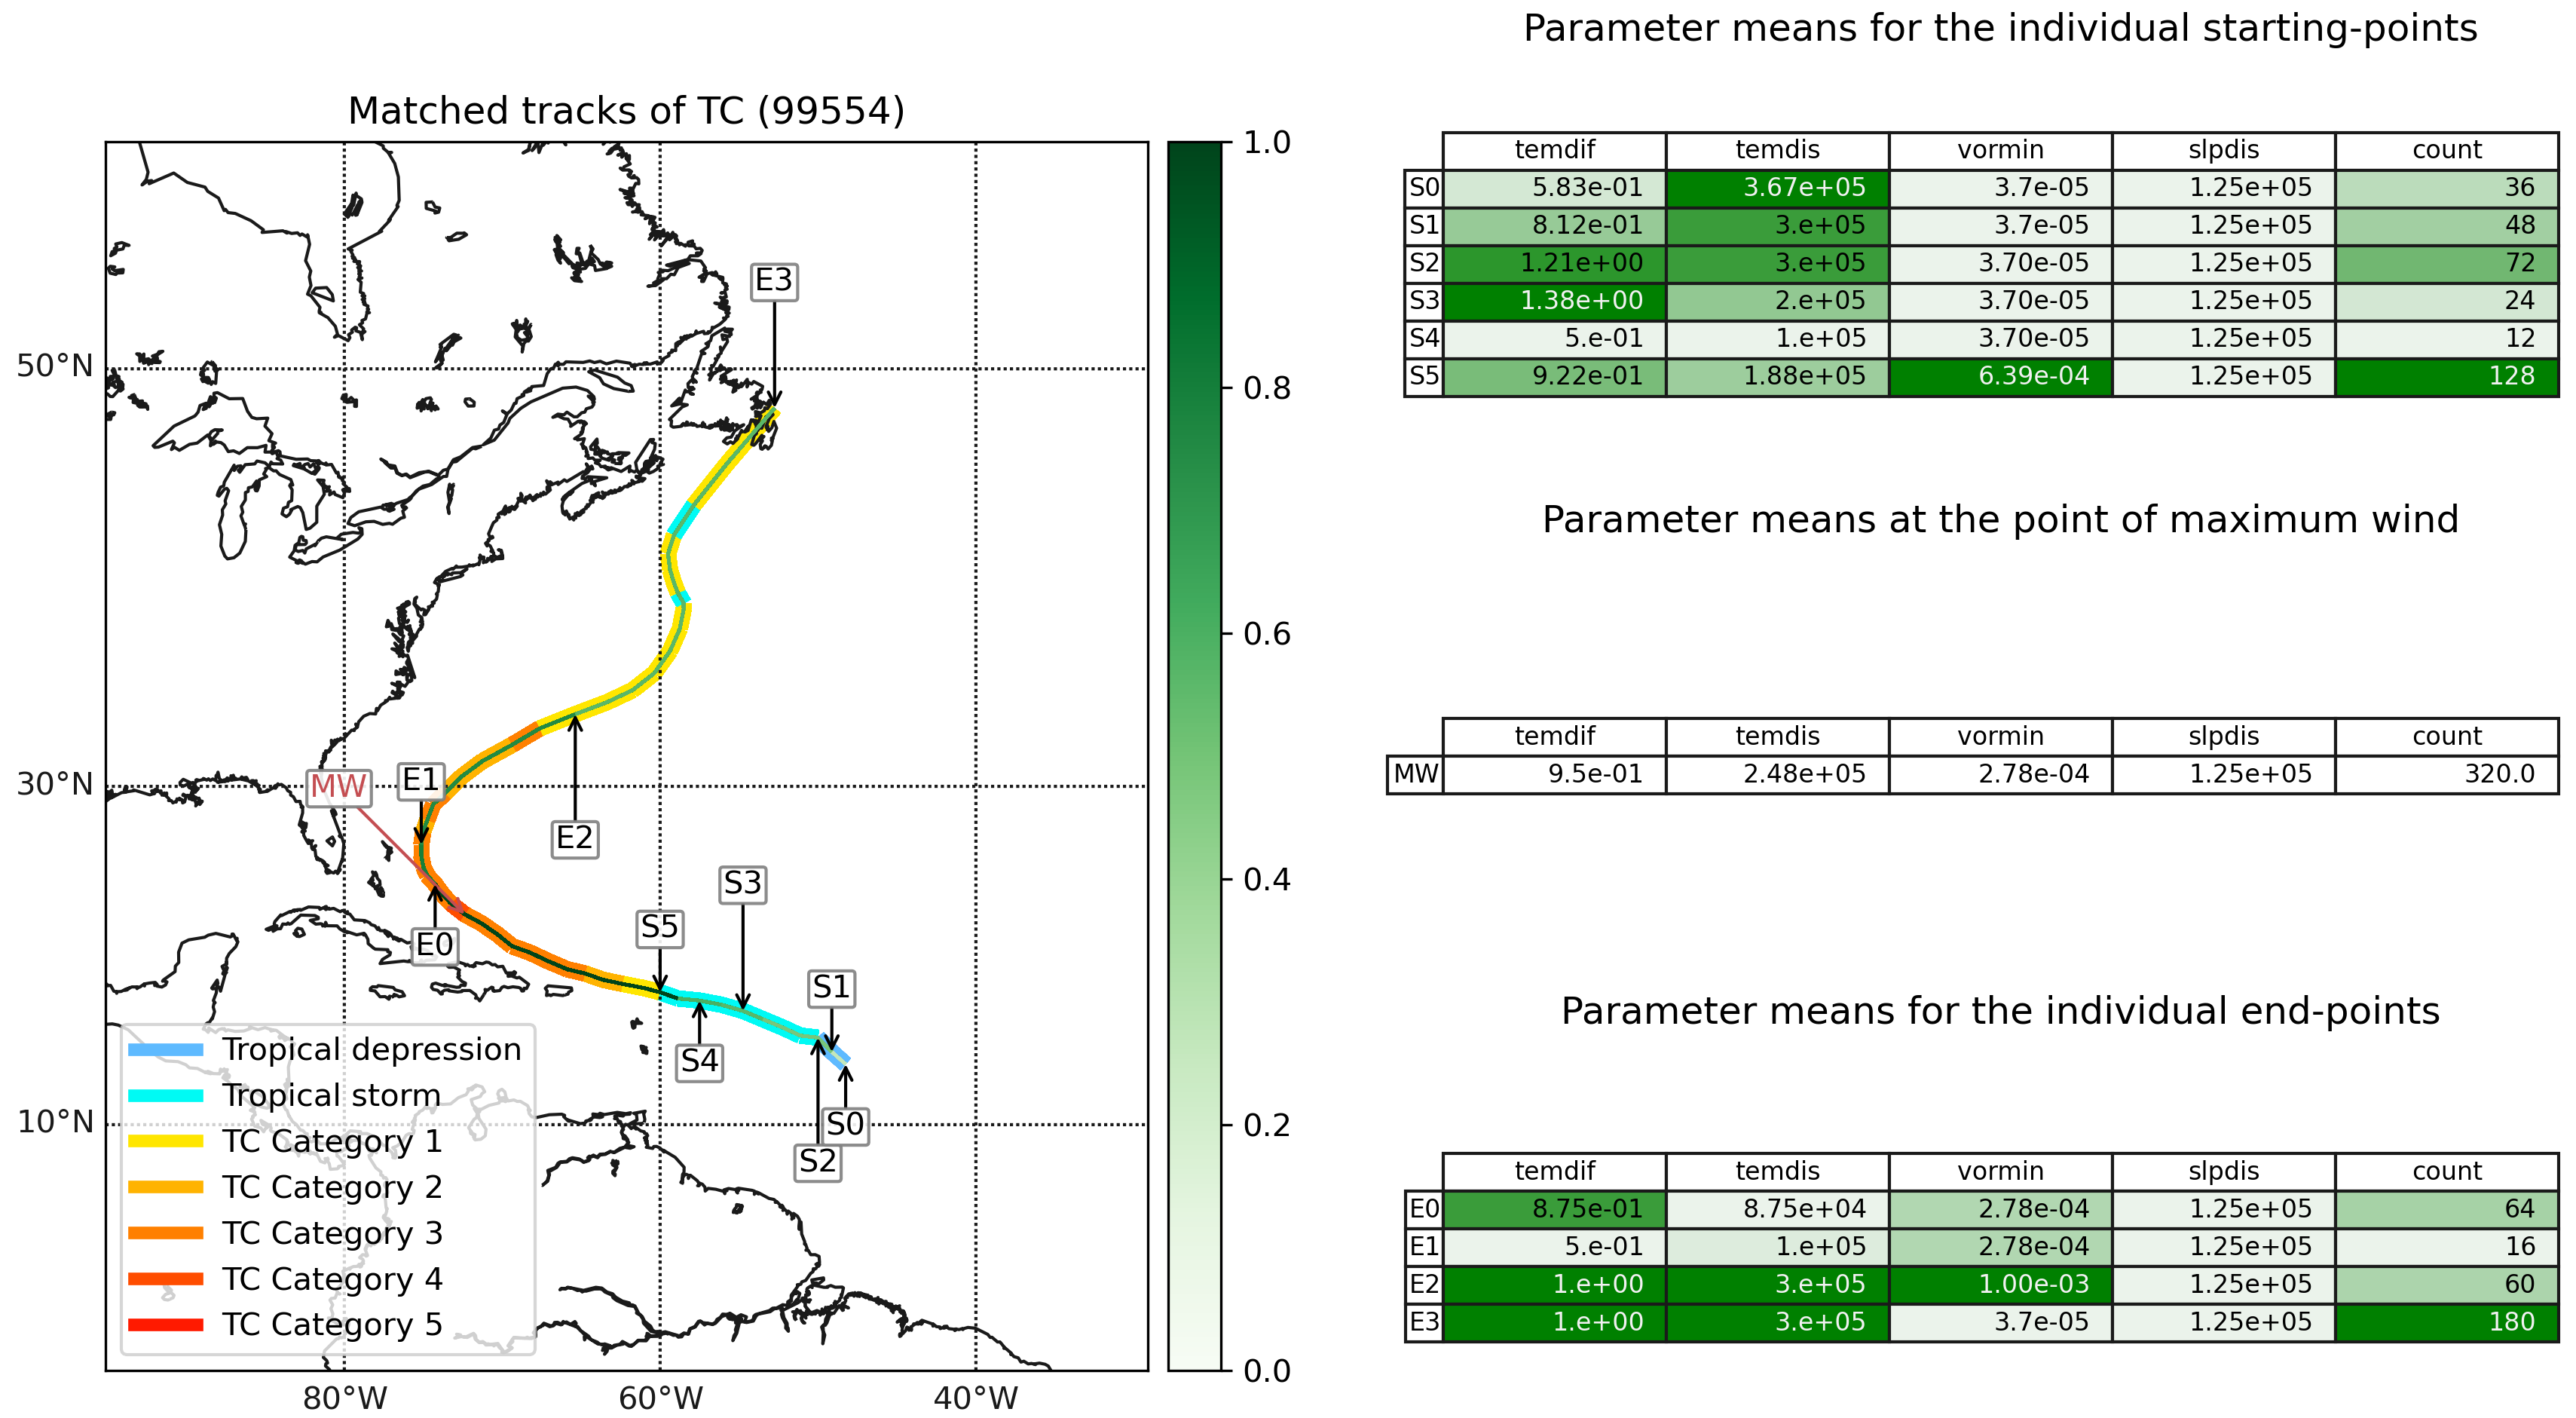
\includegraphics[width=0.9\textwidth]{img/matching_plot_ref_02_tc99554_param_id353_cat4.png}
	\caption{Tracks matching the category 4 TC (99554). The inner colour shows how many parameter combinations found the specific track segment and the background colour is set according to the current TC intensity. The start- (S1,S2,\dots), end-points (E1, E2,\dots) and the point of maximum wind (MW) are labeled.  \newline
	The tables on the right display the mean values of the parameters that correspond to the labeled points. The count specifies how many parameter combinations lead to tracks ending or starting at the given location. Since the tracks were matched using the point of maximum wind (MW), its mean values are those of the family of tracks. Its count shows how many of the 400 parameter combinations found the collection of tracks. The colour coding is dependent on the maximum and minimum values of each table column and differs between tables.}
	\label{fig:matching_plot_cat4}
\end{figure}
The first thing that strikes the eye is the lack of different tracks. Due to the SLP minimum-finding-procedure, all parameter combinations find the same locations and only very rarely do the tracks not fall on top of each other.   What differs strongly, however, are the start- and end-points of the tracks. Only between the start-point S5 and the end-point E0 is the track found by all parameter combinations. This is the duration of highest intensity, as expected.\newline
When considering the start-points S0--S3 and their corresponding parameter means on the right of the figure, it can be seen that the required temperature difference from the environment (temdif) is monotonically increasing while the size of the area considered as environment is decreasing. This can clearly be interpreted as an increasingly strict warm core criterion. Once again, it can be concluded that a weaker warm core criterion leads to tracking of TCs in earlier development phases. \newline
While the temperature difference required for S4 is quite low with \unit[0.5]{K}, the very restrictive temdis of \unit[100]{km} leads to a later tracking of the TC. This can be understood when considering the plot of the temperature anomaly of the same TC in Fig.~\ref{fig:tc-temp-anomaly} at the given time. At \unit[300]{hPa} which corresponds to roughly \unit[9]{km} no sufficiently strong temperature anomaly can be determined when only considering the area \unit[100]{km} away from the TC center.\newline
\begin{figure}[!htb]
	\centering
	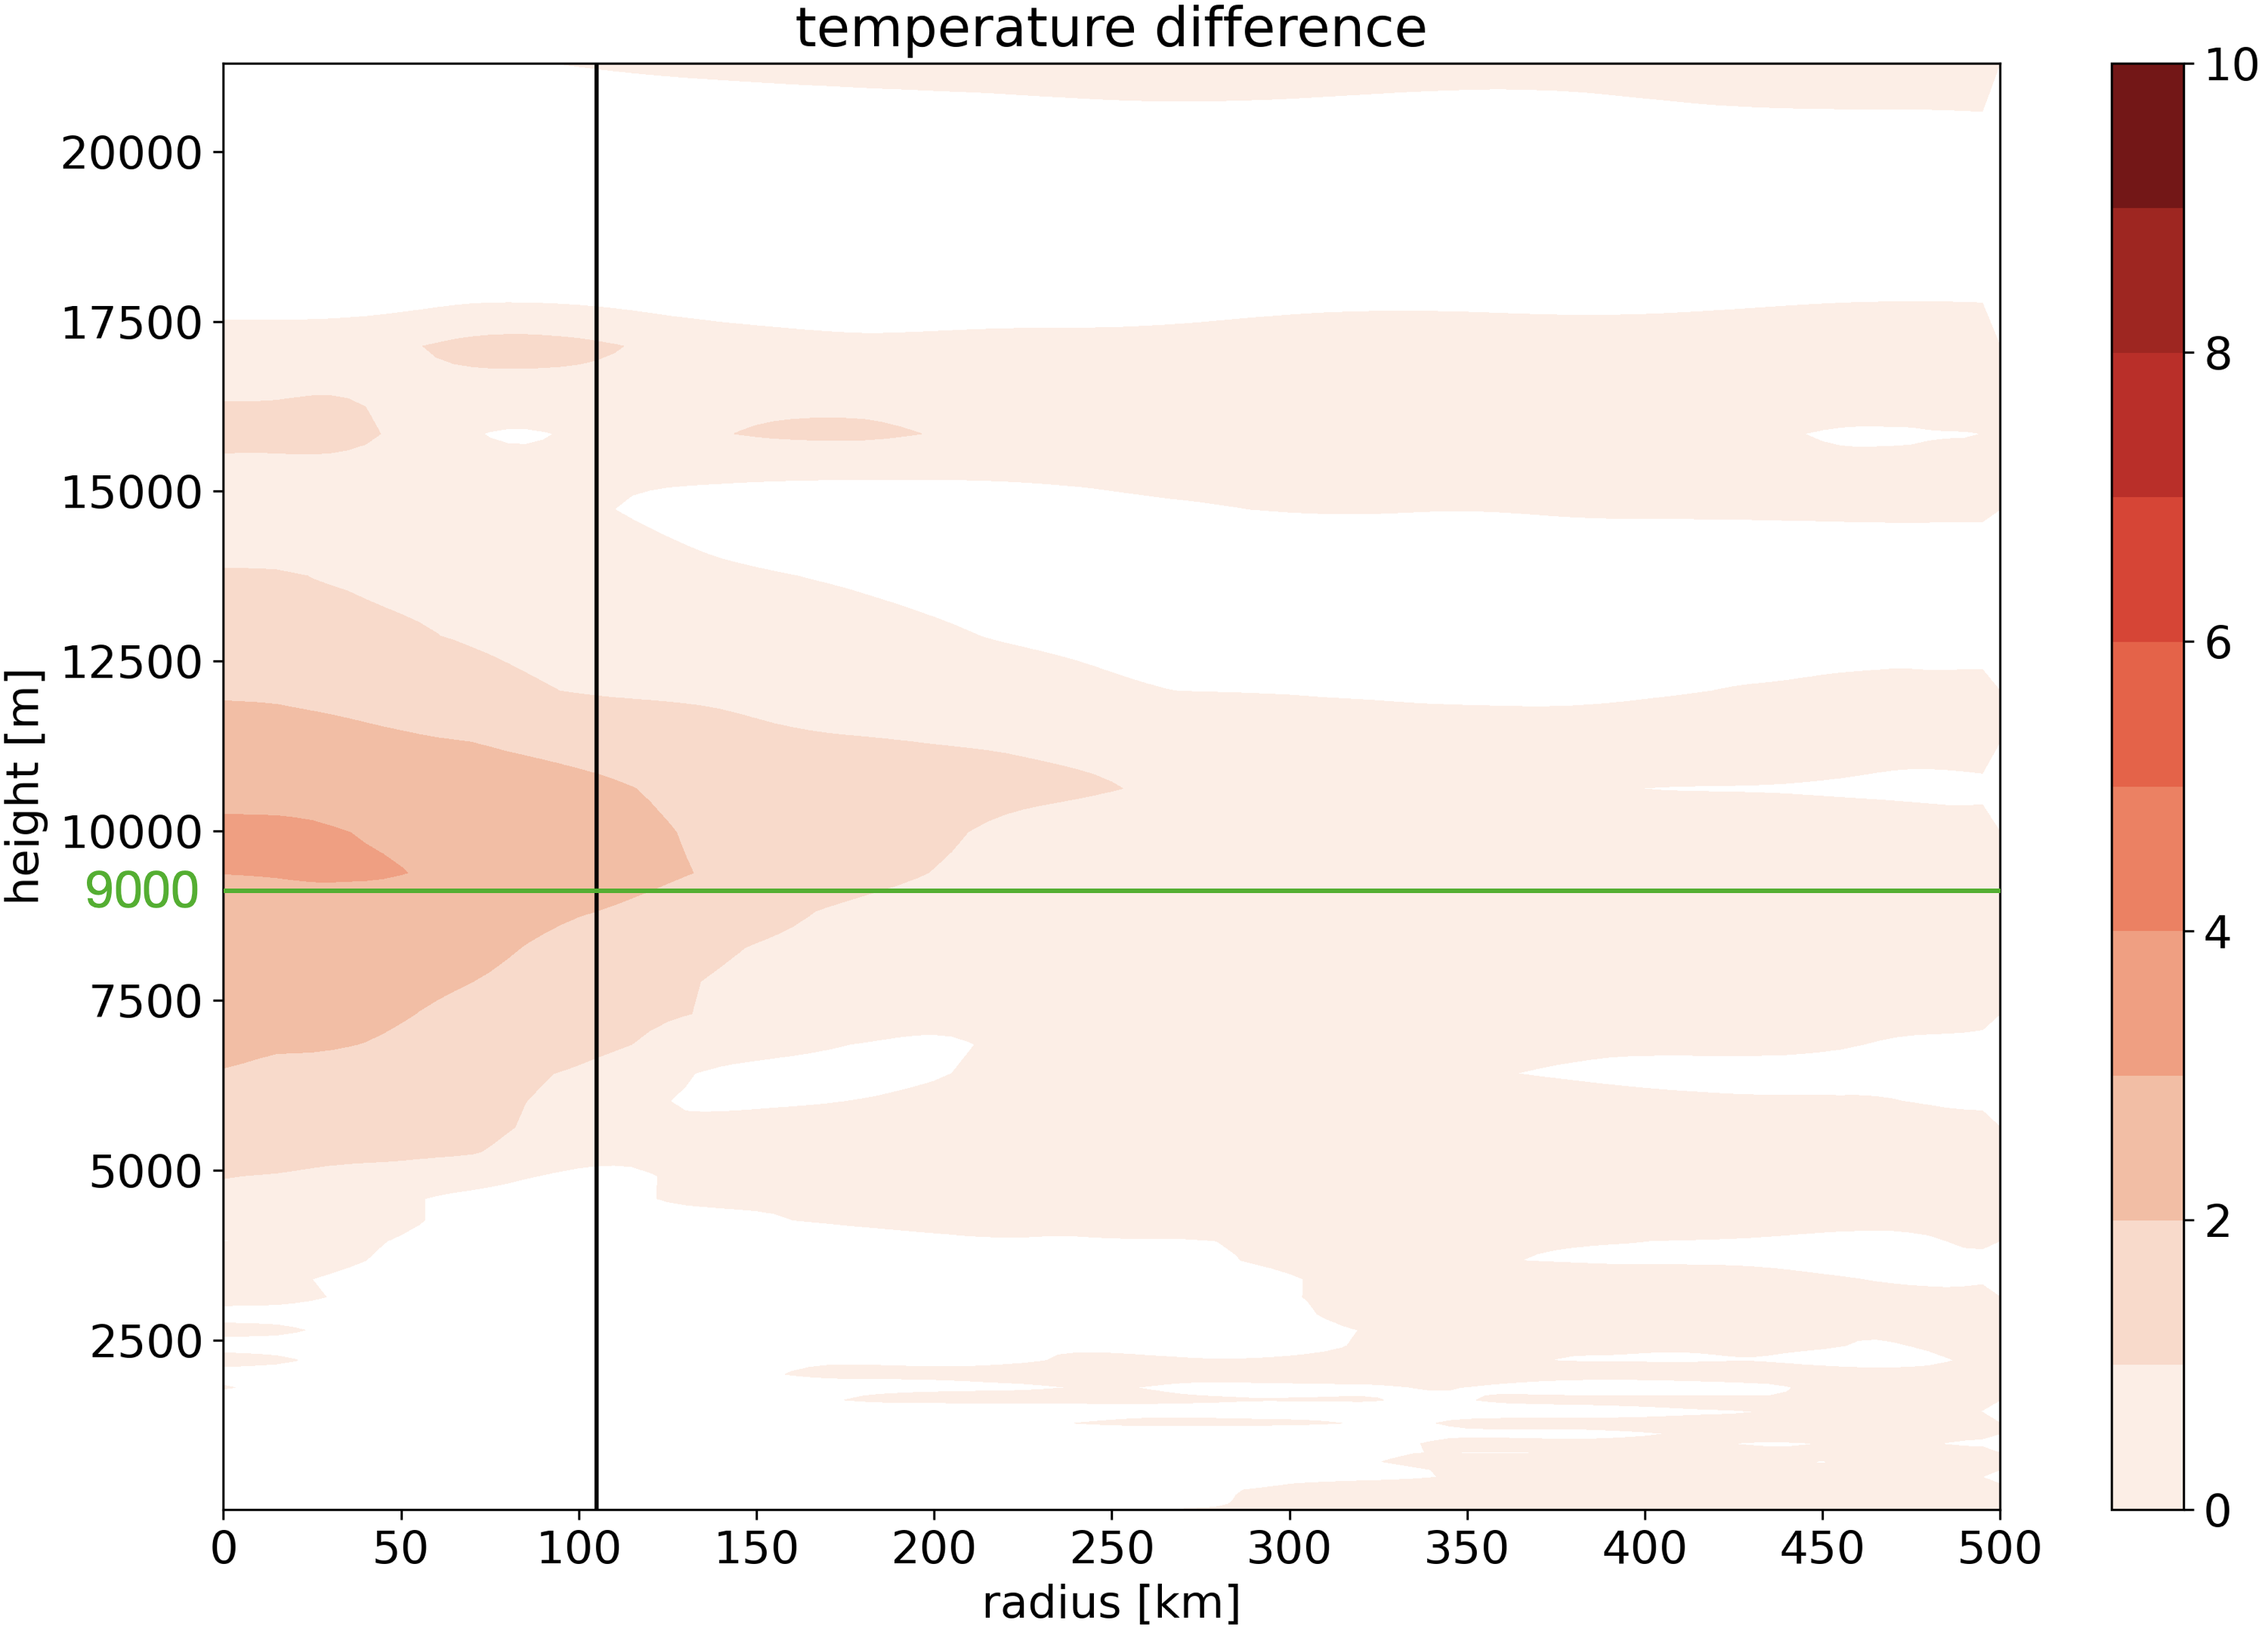
\includegraphics[width=0.7\textwidth]{img/0299554_S4temp20130902T060000Z_redo.png}
	\caption{Temperature anomaly of the TC (99554) at the point S4. The height of 9km is marked in green.}
	\label{fig:tc-temp-anomaly}
\end{figure}
The last starting point (S5) occurs at the time when the storm intensifies to a category one TC. This late detection is due to the high vorticity threshold which is more than an order of magnitude larger than for the other starting points. \newline
A similar analysis can be performed for the endpoints. We will now look a bit more closely at the parameters corresponding to the different start points.

\section{Parameter feature engineering}
The previous discussion suggests that a more general criterion might be reached through algebraic combination of different parameters. Specifically, a single warm-core criterion would be a more elegant characterisation of this physical TC property. A first naive approach was taken using Eq.~\ref{eq:warmcore}.
\begin{equation}
  \text{warmcore}_i = \frac{\text{temdif}_i}{\max_{i}\{ \text{temdif}_i\}} - 3 \times \frac{\text{temdis}_i}{\max_i\{ \text{temdis}_i\}}
  \label{eq:warmcore}
\end{equation}
With the goal of relating the two parameters temdif and temdis, both were first max-normalised. Furthermore, due to their physical meanings, the new warm-core criterion has to be proportional to temdif and inversely proportional to temdis. A more pronounced temperature anomaly leads to a stronger warm core criterion. A larger area that is used to calculate the environment temperature on the other hand, poses a weaker requirement to the warm core of the TC. Finally, the factor three on the temdis term was determined through trial and error.
Fig.~\ref{fig:clustering} shows a plot of the relationship between the vorticity and the new warm-core criterion for the different start-points. Although the clustering is in no way satisfactory, it can be seen that the means of the warm-core criterion of points S0-S4 are increasing. Furthermore, with a combination of the minimum vorticity threshold with the new warm-core criterion S5 can be easily separated from the other locations. Further feature engineering might prove fruitful.

\begin{figure}[!htb]
	\centering
	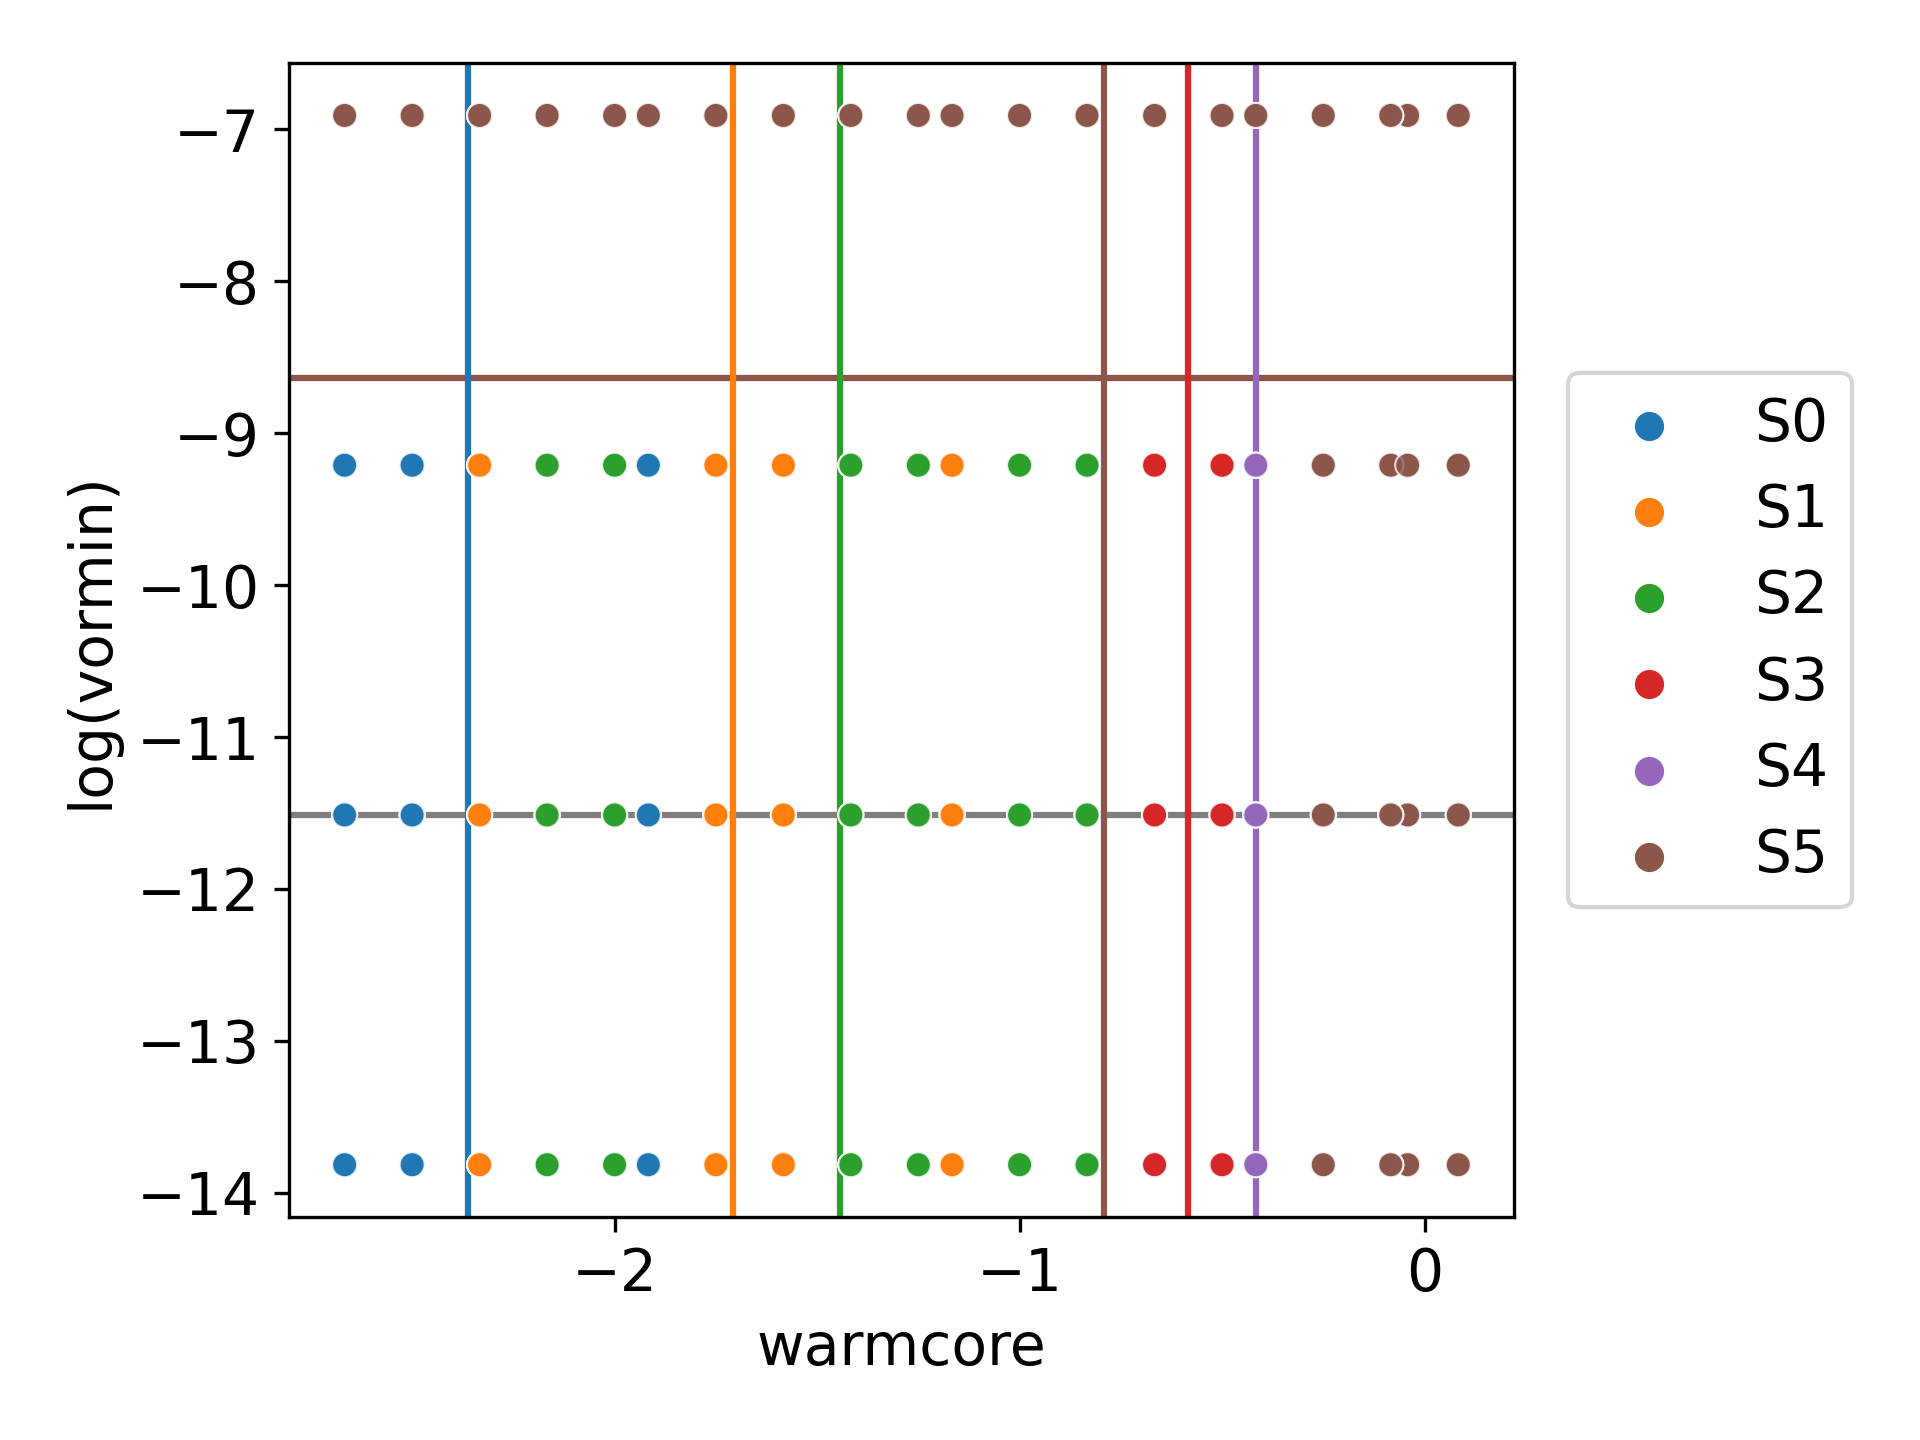
\includegraphics[width=0.7\textwidth]{img/combined_warmcore_criterion.png}
	\caption{Parameter scatterplot between the minimum vorticity and the warm core criterion from Eq.~\ref{eq:warmcore}. S1-S5 are the starting points of the TC with tc\_id 99554. The horizontal and vertical lines show the respective parameter means of the start-points. The horizontal grey line is the mean of start-points S0-S4.}
	\label{fig:clustering}
\end{figure}

\section{Analysis of an interrupted track}
Originally, the parameters from Tab.~\ref{tab:orig-params} were usually used to track TCs.
\begin{table}[!htb]
	\centering
	\begin{tabular}{|l|l|l|}
		\hline
		\textbf{parameter} & \textbf{unit} & \textbf{values} \\ \hline
		temdif             & K             & 1     \\
		temdis             & km             & 200          \\
		slpdis             & km             & 100          \\
		vormin             & 1/s           & $10^{-5}$
		\\
		\hline
	\end{tabular}
	\caption{Original parameter combination}
	\label{tab:orig-params}
\end{table}
Consequently, 58 plots with matched tracks were created from base TCs that were found using the original parameters. They can be found in the supplementary information. One peculiarity of these plots is that occasionally the point of maximum wind of the base TC is not the actual point of maximum wind of the family of tracks. An exemplary incident is depicted in Fig.~\ref{fig:interrupted-track}. 
\begin{figure}[!htb]
	\centering
	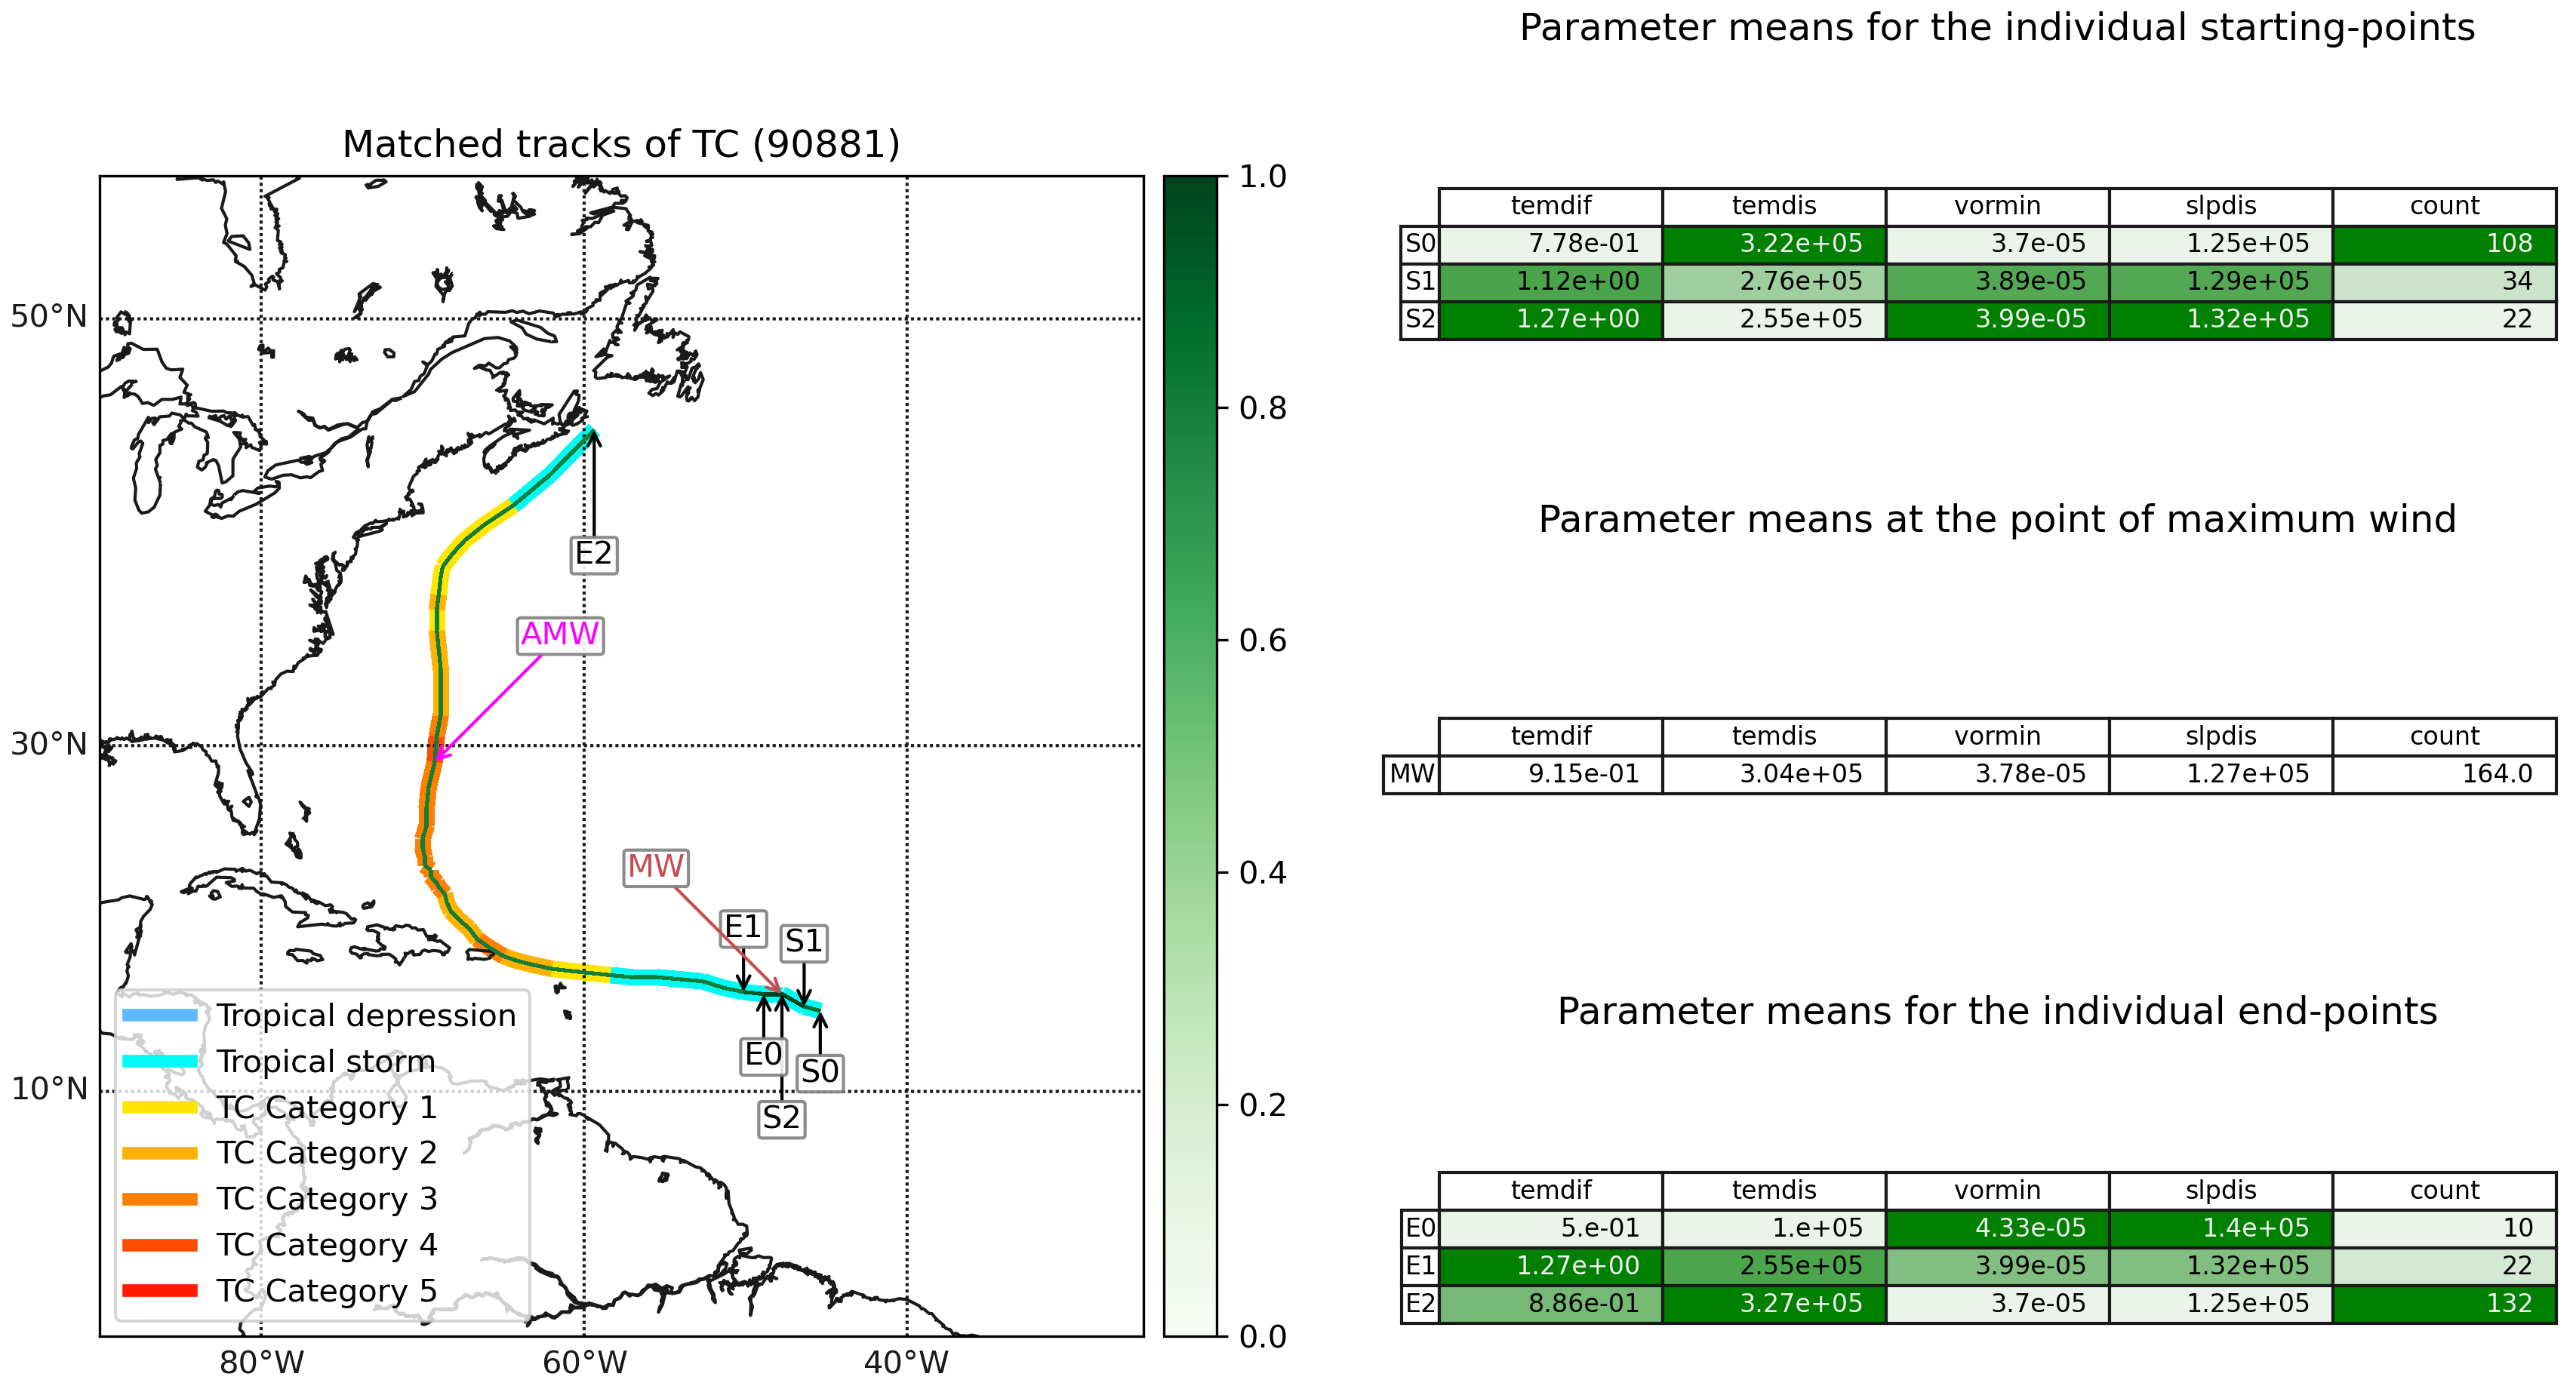
\includegraphics[width=0.9\textwidth]{img/matching_plot_reasonable_amw_ref_04_tc90881_param_id149_cat0.png}
	\caption{An interrupted track where the actual radius of maximum wind (AMW) is different from the radius of maximum wind (MW) of the base TC used for the track matching.}
	\label{fig:interrupted-track}
\end{figure}
The original parameter combination only tracks the TC up to E1. This is unfortunate since the actual point of maximum wind is much later. The original parameters therefore loose the TC before it intensifies to category four. Most likely, the TC would have been found later again. However, the track is interrupted and incorrectly identified as two different TCs. This shows the great potential of the parameter variation approach. By allowing different thresholds and matching the tracks in retrospective, the TC is tracked over its entire lifetime. The next step should be to use these techniques automatically on all tracks and to filter out tracks that not sufficiently many parameters agree on. 